\documentclass[a4paper,12pt]{report}
\usepackage{graphicx}
\usepackage{hyperref}
\usepackage[T1]{fontenc}
\usepackage[utf8]{inputenc}
\usepackage{array}
\usepackage{setspace}
\usepackage[paper=a4paper,margin=1in]{geometry}
\usepackage[section]{placeins}


\begin{document}
    
    \begin{titlepage}
        
        \noindent
        \begin{minipage}[t]{0.19\textwidth}
            \vspace{-4mm}{
\includegraphics[scale=1.15]{image/logo-unimib.pdf}}
        \end{minipage}
        \begin{minipage}[t]{0.81\textwidth}
        {
                \setstretch{1.42}
                {\textsc{Università degli Studi di Milano - Bicocca}} \\
                \textbf{Scuola di Scienze} \\
                \textbf{Dipartimento di Informatica, Sistemistica e Comunicazione} \\
                \textbf{Corso di laurea in Informatica} \\
                \par
        }
        \end{minipage}
        
	\vspace{55mm}
        
	\begin{center}
            {\LARGE{
                    \setstretch{1.2}
                    \textbf{Relazione Finale del Progetto d'Esame\\ del corso di Ingegneria del Software \\ Brew-Day! }
                    \par
            }}
        \end{center}
        
        \vspace{50mm}
        
        \begin{flushright}
            {\large \textbf{Componenti del gruppo:}} \\
            \large{Gilardi Alessandro - 866035} \\
            \large{Qazim Toska - 847361} \\
            \large{Refolli Francesco - 865955} \\
        \end{flushright}
        
        \vspace{40mm}
        \begin{center}
            {\large{\bf Anno Accademico 2022-2023}}
        \end{center}

        \restoregeometry
        
    \end{titlepage}
    
    \newpage
   \tableofcontents
   
   \newpage
    
    
    \chapter{Introduzione}
    
    	\section{Descrizione del Progetto}	
	Brew Day! è un'applicazione che consente ai birrai casalinghi produttori di birra "all-grain” di mantenere un database organizzato delle loro ricette di birra. Consente quindi agli utenti di creare, archiviare e modificare le ricette e successivamente eliminarle.\\
Ogni home brewer ha un'attrezzatura specifica, le cui caratteristiche portano a un particolare "batch size", il numero massimo di litri che possono essere erogati in un singolo ciclo. Le ricette prevedono l’uso di ingredienti comuni come l’acqua, malti, luppolo, lieviti, zuccheri, additivi, oltre ad ingredienti aggiuntivi che rendono la birra particolare.\\
L’applicazione memorizza le quantità degli ingredienti in una misura "assoluta", in unità per Litro, in modo da consentire una conversione diretta della ricetta quando l'apparecchiatura, e di conseguenza la dimensione del batch, viene aggiornata.\\
Oltre alle ricette effettive, l'applicazione offre la possibilità di mantenere le istanze di ricette eseguite, ovvero particolari miscele basate su una ricetta.\\
Le birre create possono essere accompagnate da note per fare riferimento a problemi che possono influire sulla birra risultante e che i birrai vorrebbero tenere registrati. Un particolare tipo di note sono le note di degustazione, che consentono ai birrai di tenere traccia delle opinioni su una birra di una particolare birra.\\
Oltre a queste funzionalità più tradizionali di Brew Day!, l'applicazione mantiene un elenco di ingredienti disponibili. Ciò consente ai birrai di essere informati sugli ingredienti mancanti per la birra successiva.\\
Un'istanza di ricetta, ovvero una particolare birra, consente agli utenti di aggiornare l'elenco degli ingredienti disponibili, sottraendo gli ingredienti utilizzati da quelli disponibili.\\
Brew Day! supporta la funzione "cosa dovrei preparare oggi?” che consiglia la ricetta che massimizza l'uso degli ingredienti disponibili, tenendo conto della capacità dell'attrezzatura.
Per informazioni sull'installazione e uso dell'applicazione è possibile visitare la sezione \href{https://github.com/lta-unimib/progetto-brew-day-1-brew-day-birra/wiki}{Wiki su gitHub}.

\newpage
    	\section{Processo Adottato}	
	E' stato adottato il Framework Scrum al fine tenere sotto controllo lo stato di avanzamento del progetto, ispezionando frequentemente il lavoro fatto per verificare che si stia procedendo verso gli obiettivi posti e, nel caso si stia deviando dagli obiettivi, fare delle correzioni. \\
Abbiamo deciso di effettuare 4 sprint, ognuno della durata di 5 giorni.\\
Sono state svolte le seguenti attività:
	\begin{itemize}
		\item Meeting iniziale, il primo giorno, in cui abbiamo creato la Product Backlog e il Gantt (figure \ref{fig:scrum1}, \ref{fig:scrum2}, \ref{fig:scrum3}, \ref{fig:scrum4} )
		\item	Sprint Planning, all’inizio di ogni Sprint, in cui abbiamo pianificato la Sprint Backlog e identificato lo Sprint Goal
		\item Daily Scrum, meeting online giornaliero di 15 minuti in cui ci siamo confrontati sul lavoro svolto il giorno precedente e pianificato i compiti del giorno per il raggiungimento dello Sprint Goal
		\item Sprint Review e Sprint Retrospective, al termine di ogni Sprint, in cui abbiamo ispezionato il lavoro svolto, valutato se l’obiettivo prefissato è stato raggiunto e con quali risultati e infine valutato cosa continuare a fare, cosa smettere di fare e cosa migliorare nello sprint successivo per ottenere performance ancora più efficienti.
	\end{itemize}
La qualità del codice è stata monitorata utilizzando i tool Understand e SonarQube, oltre a SonarCloud.	

	\begin{figure}[!h]
		\centering
		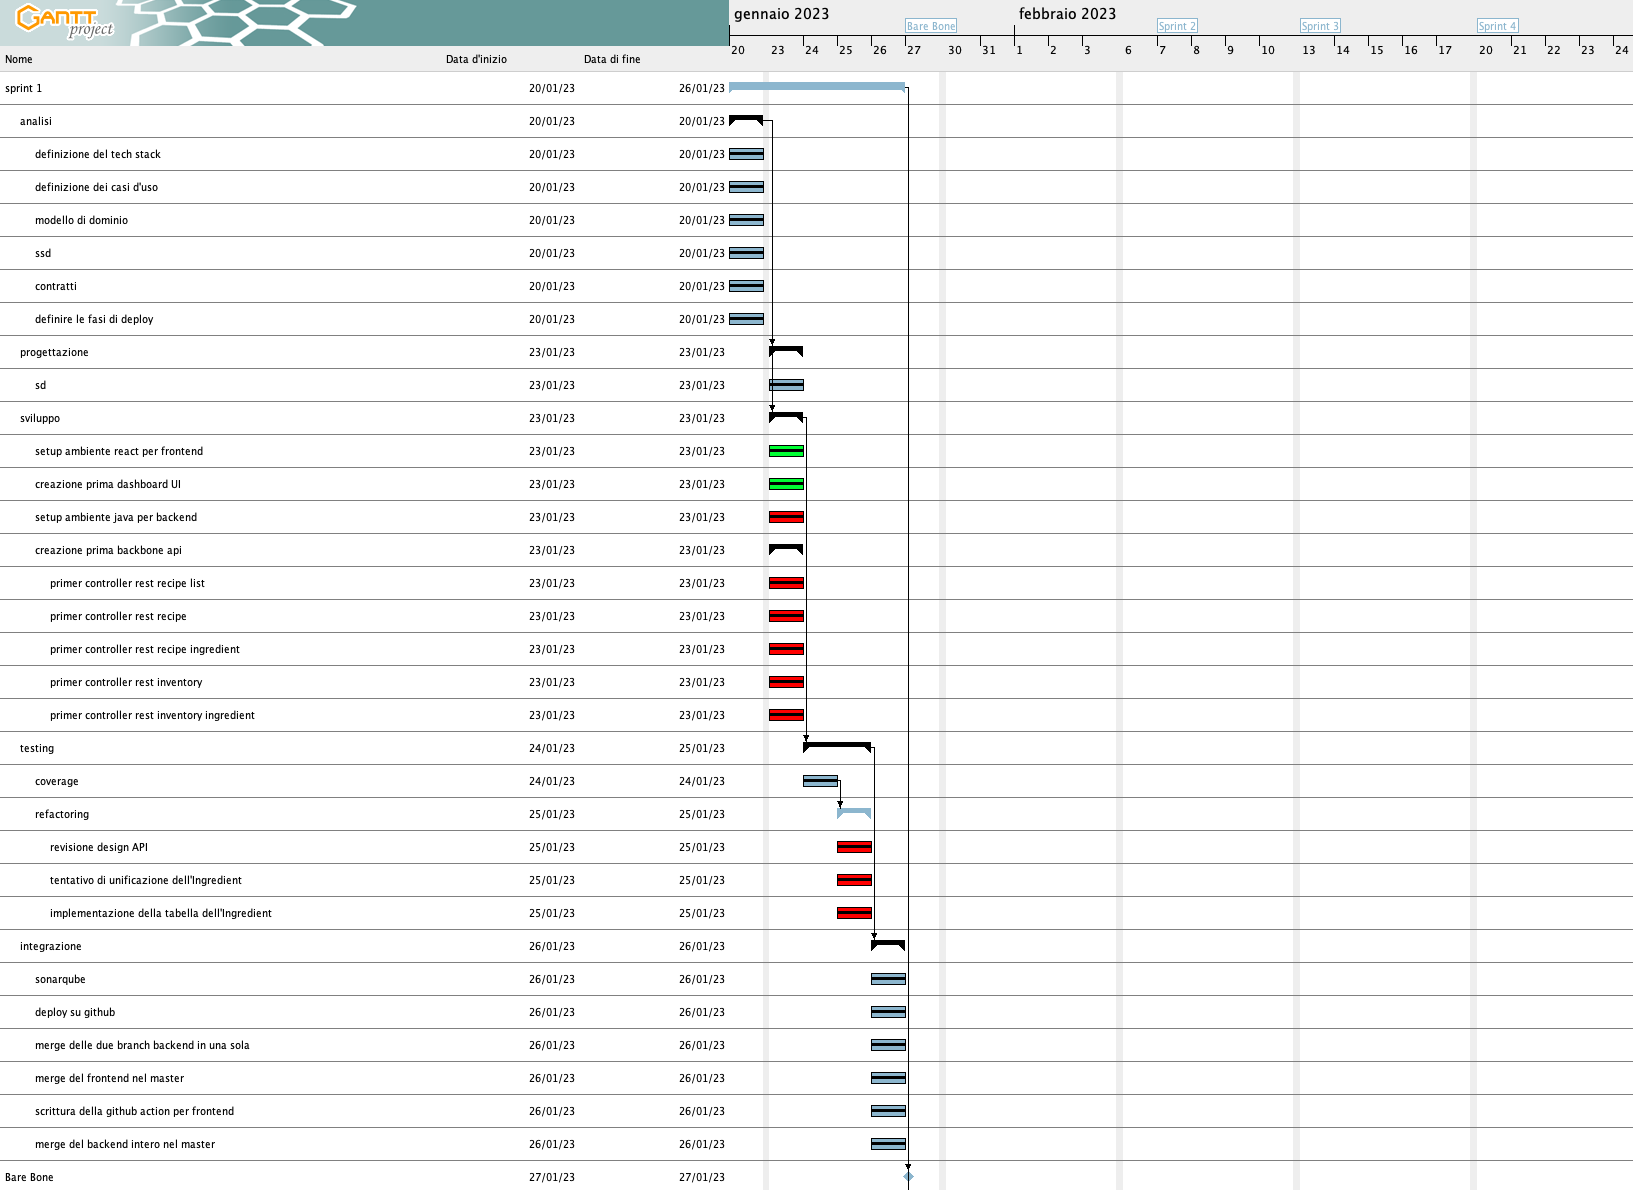
\includegraphics[width=0.9\linewidth]{image/scrum1.png}
		\caption{Gantt - Sprint 1}\label{fig:scrum1}
	\end{figure}

	\begin{figure}[!h]
		\centering
		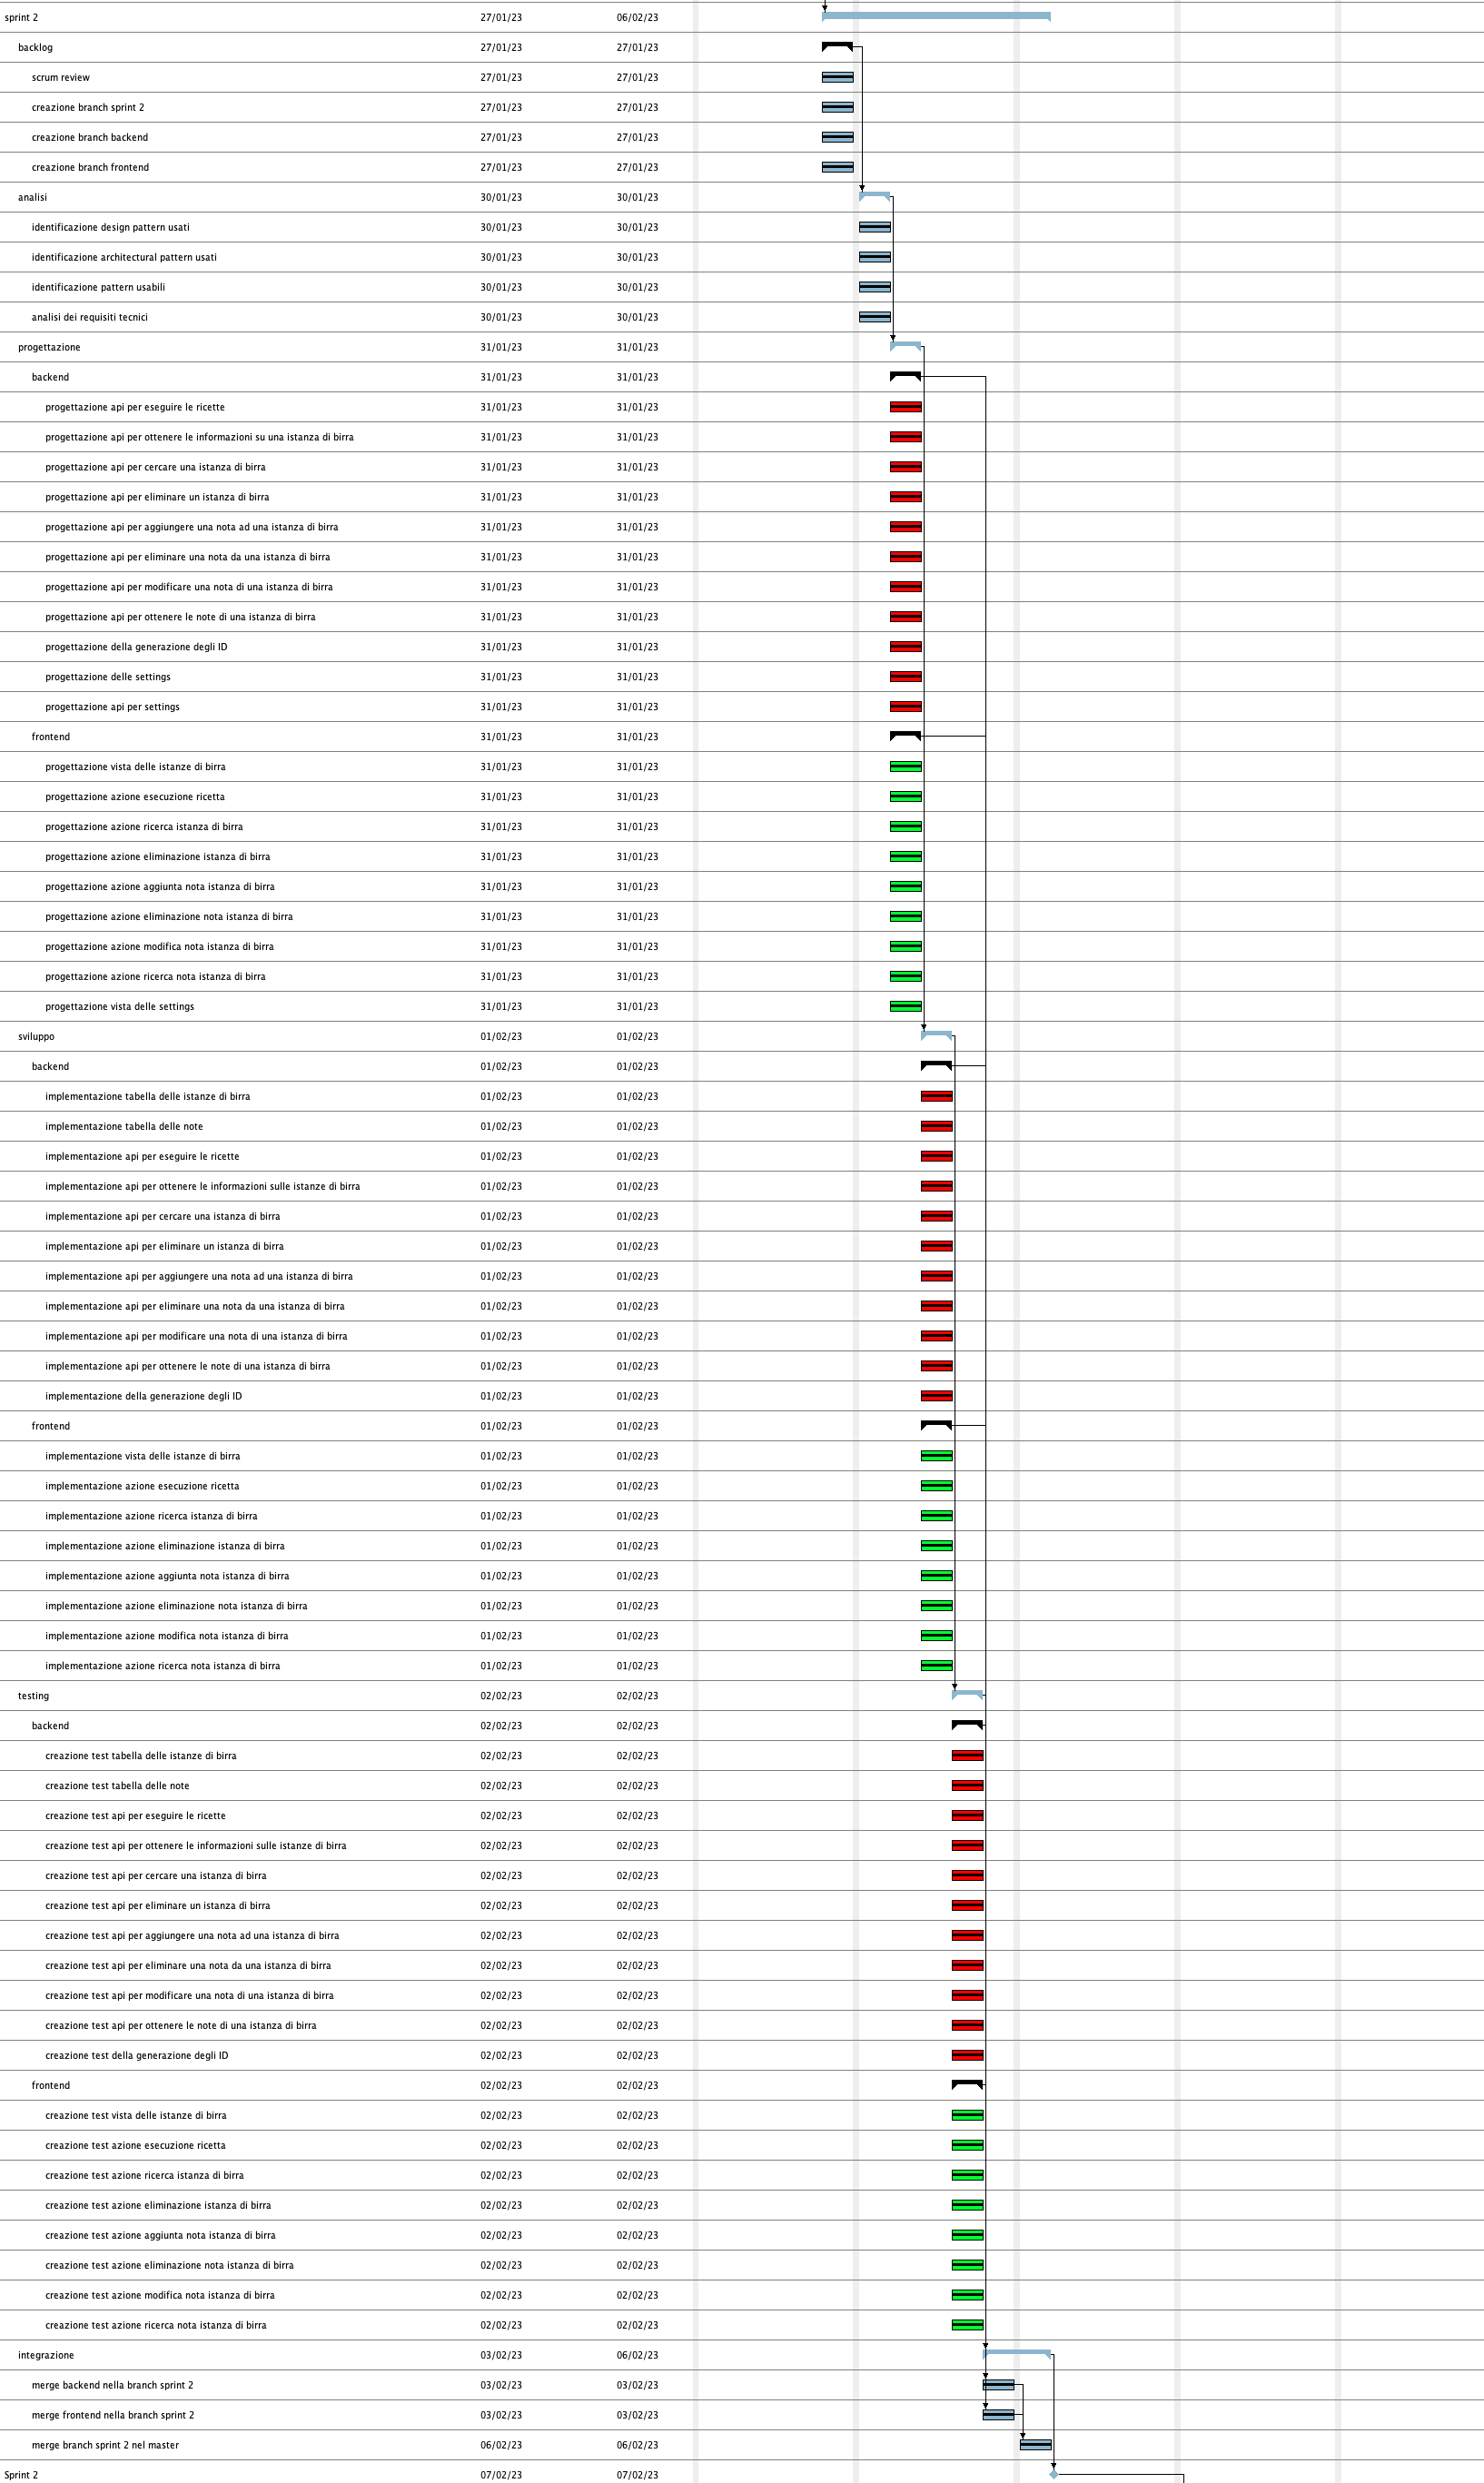
\includegraphics[width=0.9\linewidth]{image/scrum2.png}
		\caption{Gantt - Sprint 2}\label{fig:scrum2}
	\end{figure}
	
	\begin{figure}[!h]
		\centering
		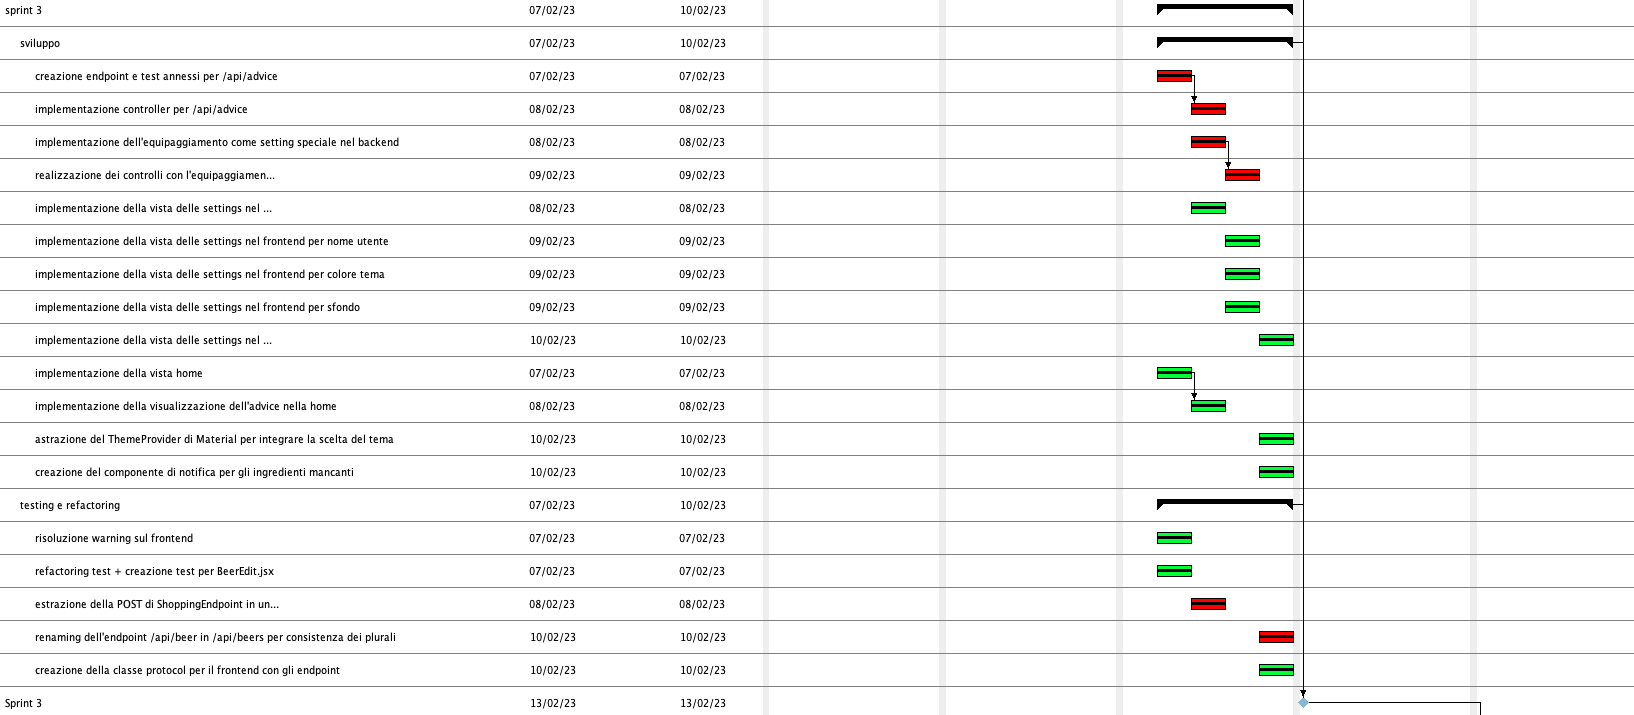
\includegraphics[width=0.9\linewidth]{image/scrum3.png}
		\caption{Gantt - Sprint 3}\label{fig:scrum3}
	\end{figure}
	
	\begin{figure}[!h]
		\centering
		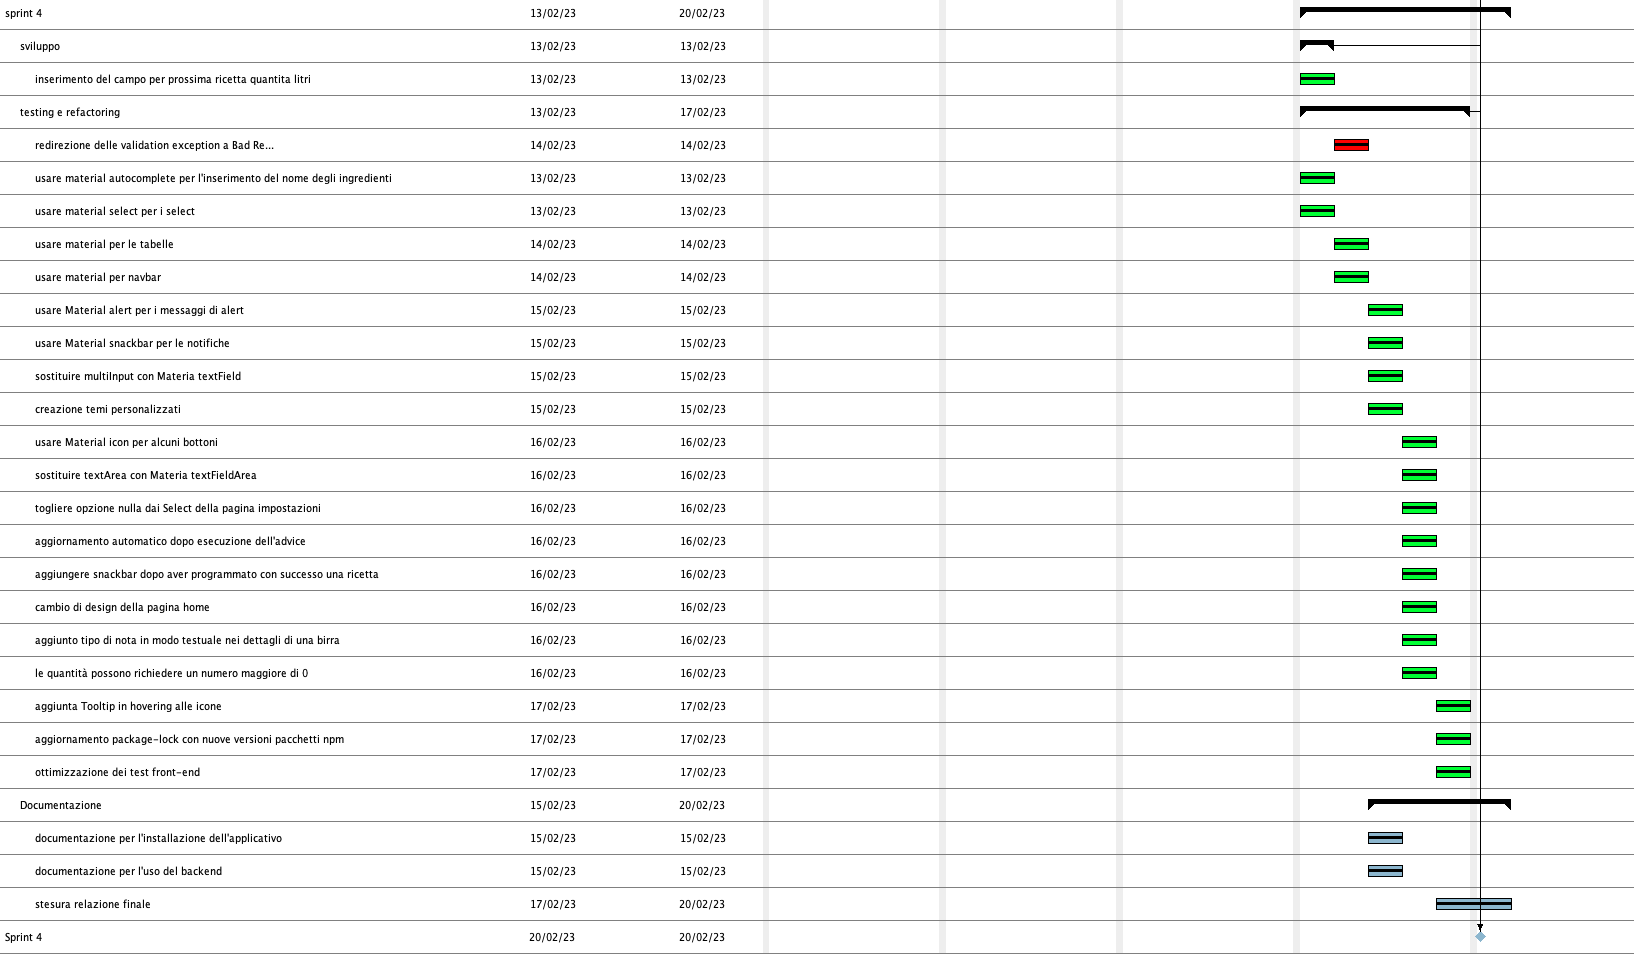
\includegraphics[width=0.9\linewidth]{image/scrum4.png}
		\caption{Gantt - Sprint 4}\label{fig:scrum4}
	\end{figure}

    	\section{Utilizzo di GitHub}
Per tenere traccia dell'attività e dello stato di avanzamento del progetto abbiamo utilizzato gitHub:
\begin{itemize}
		\item Per ciascuno Sprint abbiamo definito una milestone che la caratterizza
		\item Per ogni attività di sviluppo abbiamo definito una issue che la descriva, all'interno della corrispondente milestone
		\item Abbiamo fatto ampio uso dei branch per lavorare su soluzioni parziali o questioni più ampie
		\item Sono state utilizzate le GitHub Action per automatizzare la fase di test, build e analisi con SonarCloud
		\item E' stato utilizzato il task Tracker offerto da gitHub nella sezione Project per condividere i progressi effettuati tra i componenti del gruppo
		\item E' stata adottata la seguente strategia di gestione del branch (figura \ref{fig:branchStrategy}): una branch master, con il codice stabile; una branch per ogni sprint (associato ad una milestone), da cui si forkano le varie branch che contengono le feature della milestone; ogni k merge / commit sulla branch di sprint si rilascia una preview sul master
	\end{itemize}

	\begin{figure}[!h]
		\centering
		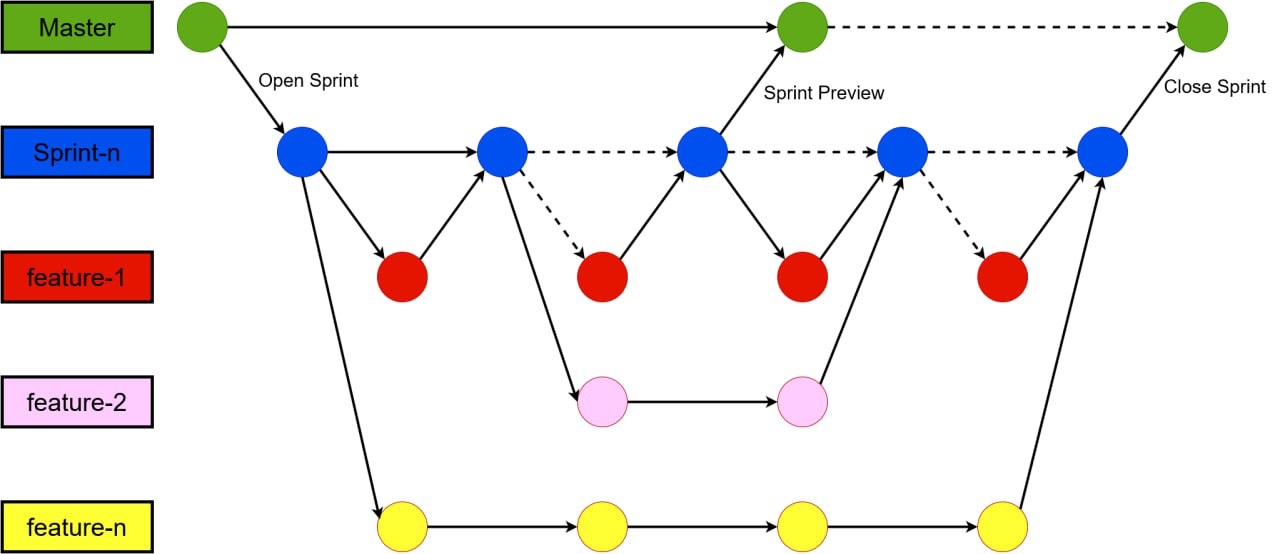
\includegraphics[width=0.9\linewidth]{image/branchStrategy.png}
		\caption{Branch Strategy}\label{fig:branchStrategy}
	\end{figure}
	
\newpage
    \chapter{Analisi}
    	\section{Glossario}
	All'inizio del progetto è stato realizzato il glossario riportato nella tabella \ref{tab:Gloassario}.
    		\begin{table}[!h]
      			\renewcommand{\arraystretch}{1.2}
      			\begin{tabular}{p{0.2\textwidth}|p{0.7\textwidth}} 
        				\textbf{Nome}  & \textbf{Descrizione} \\
    				\hline
           			birraio & un utente \\
                        		equipaggiamento & bollitore, fermentatore, pipa da birra \\
                            	capacita' & quantita' in litri che un equipaggiamento puo' supportare in una turnata \\
                          	ingrediente & malto, luppolo, lievito, zucchero, acqua, additivi \\
                          	ricetta & collezione di ingredienti con associata una quantita' \\
                          	inventario & collezione di ingredienti che l'home brewer ha a disposizione \\
                            	consiglio & ricetta che massimizza l'uso degli ingredienti nell'inventario \\
                            	istanza di birra & anche chiamata `istanza di ricetta` nel testo, birra prodotta con una certa ricetta \\
        			\end{tabular}
        			\caption{Glossario}
      			\label{tab:Gloassario}
    		\end{table}
\newpage
	\section{Requisiti Funzionali}
	All'inizio del progetto sono stati individuati i requisiti funzionali, a ciascuno dei quali è stata attribuita un'importanza, come prevede la tecnica MoSCoW (tabella \ref{tab:Requisiti-Funzionali}).
    		\begin{table}[!h]
      			\renewcommand{\arraystretch}{1.2}
      			\begin{tabular}{p{0.8\textwidth}|p{0.1\textwidth}} 
        				\textbf{Requisito}  & \textbf{MoSCoW} \\
    				\hline
                                  il sistema deve permettere all'utente di mantenere, aggiornare, eliminare ricette & M \\
                                  il sistema deve permettere all'utente di mantenere l'inventario & M \\
                                  il sistema deve permettere all'utente di indicare che una ricetta e' stata eseguita e quindi aggiornare l'inventario di conseguenza & M \\
                                  il sistema deve permettere all'utente di indicare che ha fatto la spesa e quindi aggiornare l'inventario di conseguenza & M \\
                                  il sistema deve permettere all'utente di produrre la lista della spesa per gli ingredienti mancanti di una ricetta & M \\
                                  il sistema deve permettere all'utente di generare un consiglio per la prossima birra & M \\
                                  il sistema deve permettere all'utente di mantenere le istanze di una ricetta & M \\
                                  il sistema deve permettere all'utente di aggiungere, aggiornare, eliminare note alle istanze di una birra & M \\
                                  il sistema deve notificare l'utente quando mancano degli ingredienti per la prossima birra & M \\
        			\end{tabular}
        			\caption{Requisiti Funzionali}
      			\label{tab:Requisiti-Funzionali}
    		\end{table}

\newpage
	\section{Requisiti non funzionali}
	Oltre ai requisiti funzionali, abbiamo individuato anche quelli non funzionali (tabella \ref{tab:Requisiti-Non-Funzionali}). 
    		\begin{table}[!h]
      			\renewcommand{\arraystretch}{1.2}
      			\begin{tabular}{p{0.8\textwidth}|p{0.1\textwidth}} 
        				\textbf{Requisito}  & \textbf{MoSCoW} \\
    				\hline
                                  il sistema deve mantenere le quantità degli ingredienti nelle ricette (e nell'inventario) in termini di unita' assolute (anche diverse), in modo che sia più semplice calcolare i multipli & M \\
                                  il sistema deve supportare le note normale e le note di sapore per le istanze di una ricetta  & M \\
                                  il suggerimento della birra deve massimizzare l'uso di ingredienti e equipaggiamento & M \\
                                  il sistema può supportare la possibilità di aggiungere immagini alle istanze di birra & C \\
                                  si deve permettere di eliminare una ricetta che ha associate delle birre prodotte & M \\
        			\end{tabular}
        			\caption{Requisiti Non Funzionali}
      			\label{tab:Requisiti-Non-Funzionali}
    		\end{table}	
	
	
    \newpage
	\section{Casi d'Uso}
	Nei primi giorni del progetto abbiamo identificato i seguenti casi d'uso sulla base dei requisiti del progetto. 
		\begin{figure}[!h]
			\centering
			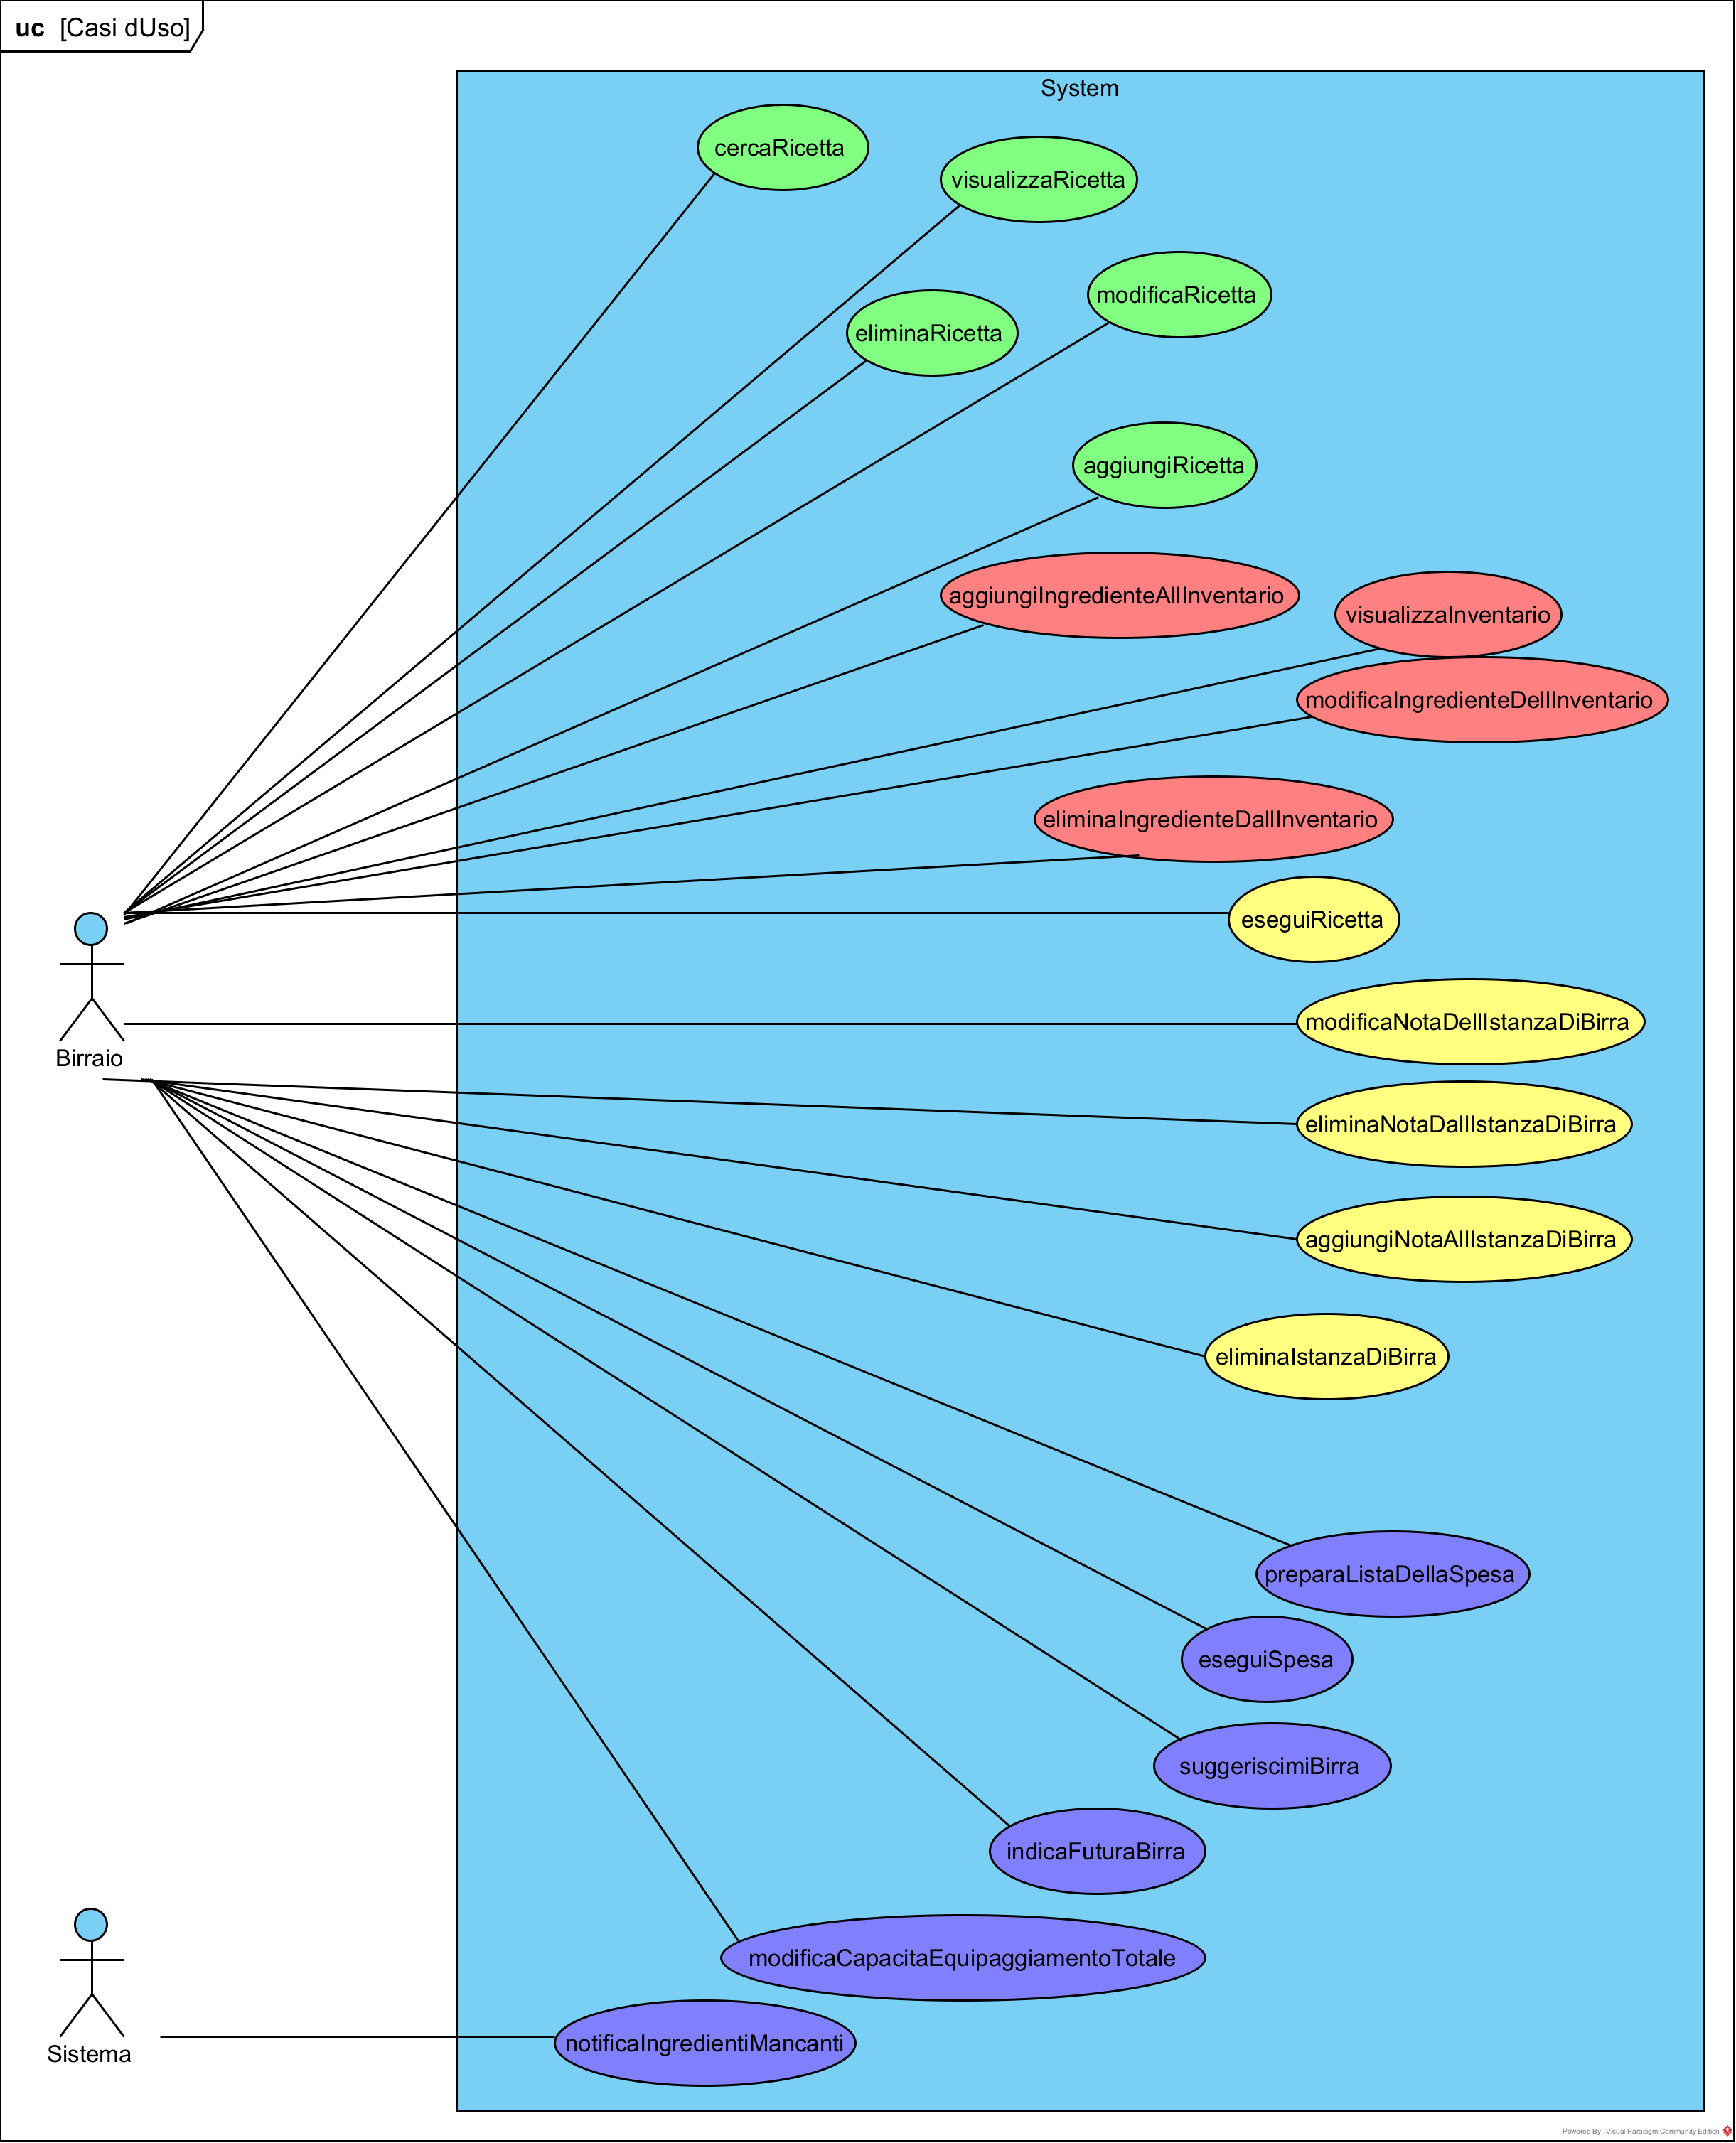
\includegraphics[width=1\linewidth]{image/Casi-dUso.png}
			\caption{Casi d'Uso}\label{fig:Casi-d'Uso}
		\end{figure}

		\subsection{Identificazione dei Casi d'Uso}
			Casi d'Uso suddivisi nelle 4 iterazioni svolte:
			\begin{enumerate}
    				\item Prima Iterazione
					\begin{itemize}
						\item aggiungiRicetta	
						\item modificaRicetta	
						\item eliminaRicetta	
						\item cercaRicetta	
						\item visualizzaRicetta	
						\item visualizzaInventario	
						\item aggiungiIngredienteAllInventario	
						\item modificaIngredienteNellInventario	
						\item eliminaIngredienteDallInventario
					\end{itemize}
    				\item Seconda Iterazione
					\begin{itemize}
						\item eseguiRicetta	
						\item eliminaIstanzaDiBirra	
						\item aggiungiNotaAllIstanzaDiBirra		
						\item eliminaNotaDallIstanzaDiBirra	
						\item modificaNotaDellIstanzaDiBirra		
					\end{itemize}			
    				\item Terza Iterazione
					\begin{itemize}
						\item eseguiSpesa	
						\item indicaFuturaBirra	
						\item preparaListaDellaSpesa	
						\item suggeriscimiBirra	
						\item notificaIngredientiMancanti	
						\item modificaCapacitaEquipaggiamentoTotale		
					\end{itemize}
				\item Quarta Iterazione - nessuno
			\end{enumerate}
		
		\subsection{Caso d'Uso in formato breve - aggiungiRicetta}
			E' stato realizzato il caso d'Uso in formato breve di aggiungiRicetta nella prima iterazione
			\begin{enumerate}
    				\item Il birraio inizia l'immissione di una nuova ricetta.
    				\item Il birraio inserisce il nome della nuova ricetta.
				\item Il birraio può inserire una descrizione della ricetta.
    				\item import caso d'uso modificaRicetta
    				\item il sistema salva la ricetta		
			\end{enumerate}		
	
		\subsection{Caso d'Uso in formato breve - modificaRicetta}		
			E' stato realizzato il caso d'Uso in formato breve di modificaRicetta nella prima iterazione
			\begin{enumerate}
    				\item Il birraio inizia la modifica di una ricetta.
    				\item while:
				\begin{enumerate}
					\item  if opt1:
						\begin{enumerate}
							\item inserisce il nome di un ingrediente
							\item inserisce la quantita' dell'ingrediente
						\end{enumerate}		
					\item  if opt2:
						\begin{enumerate}
							\item individua l'ingrediente da rinominare
							\item inserisce il nuovo nome dell'ingrediente
						\end{enumerate}		
					\item  if opt3:
						\begin{enumerate}
							\item individua un ingrediente
							\item inserisce la nuova quantita' dell'ingrediente
						\end{enumerate}
 					\item  if opt4:
						\begin{enumerate}
  							\item seleziona l'ingrediente da eliminare
						\end{enumerate}	
 					\item  if opt5:
						\begin{enumerate}
  							\item inserisce il nuovo nome della ricetta
						\end{enumerate}
 					\item  if opt6:
						\begin{enumerate}
  							\item inserisce la nuova descrizione della ricetta
						\end{enumerate}	
    					\item il sistema salva la ricetta
				\end{enumerate}	
			\end{enumerate}
			
	\newpage	
	\section{Modello di Dominio}
Durante le iterazioni è stato realizzato il modello di dominio (figura \ref{fig:Modello-Dominio}), il quale fornisce una rappresentazione visuale delle classi concettuali e degli oggetti del mondo reale del dominio.
		\begin{figure}[!h]
			\centering
			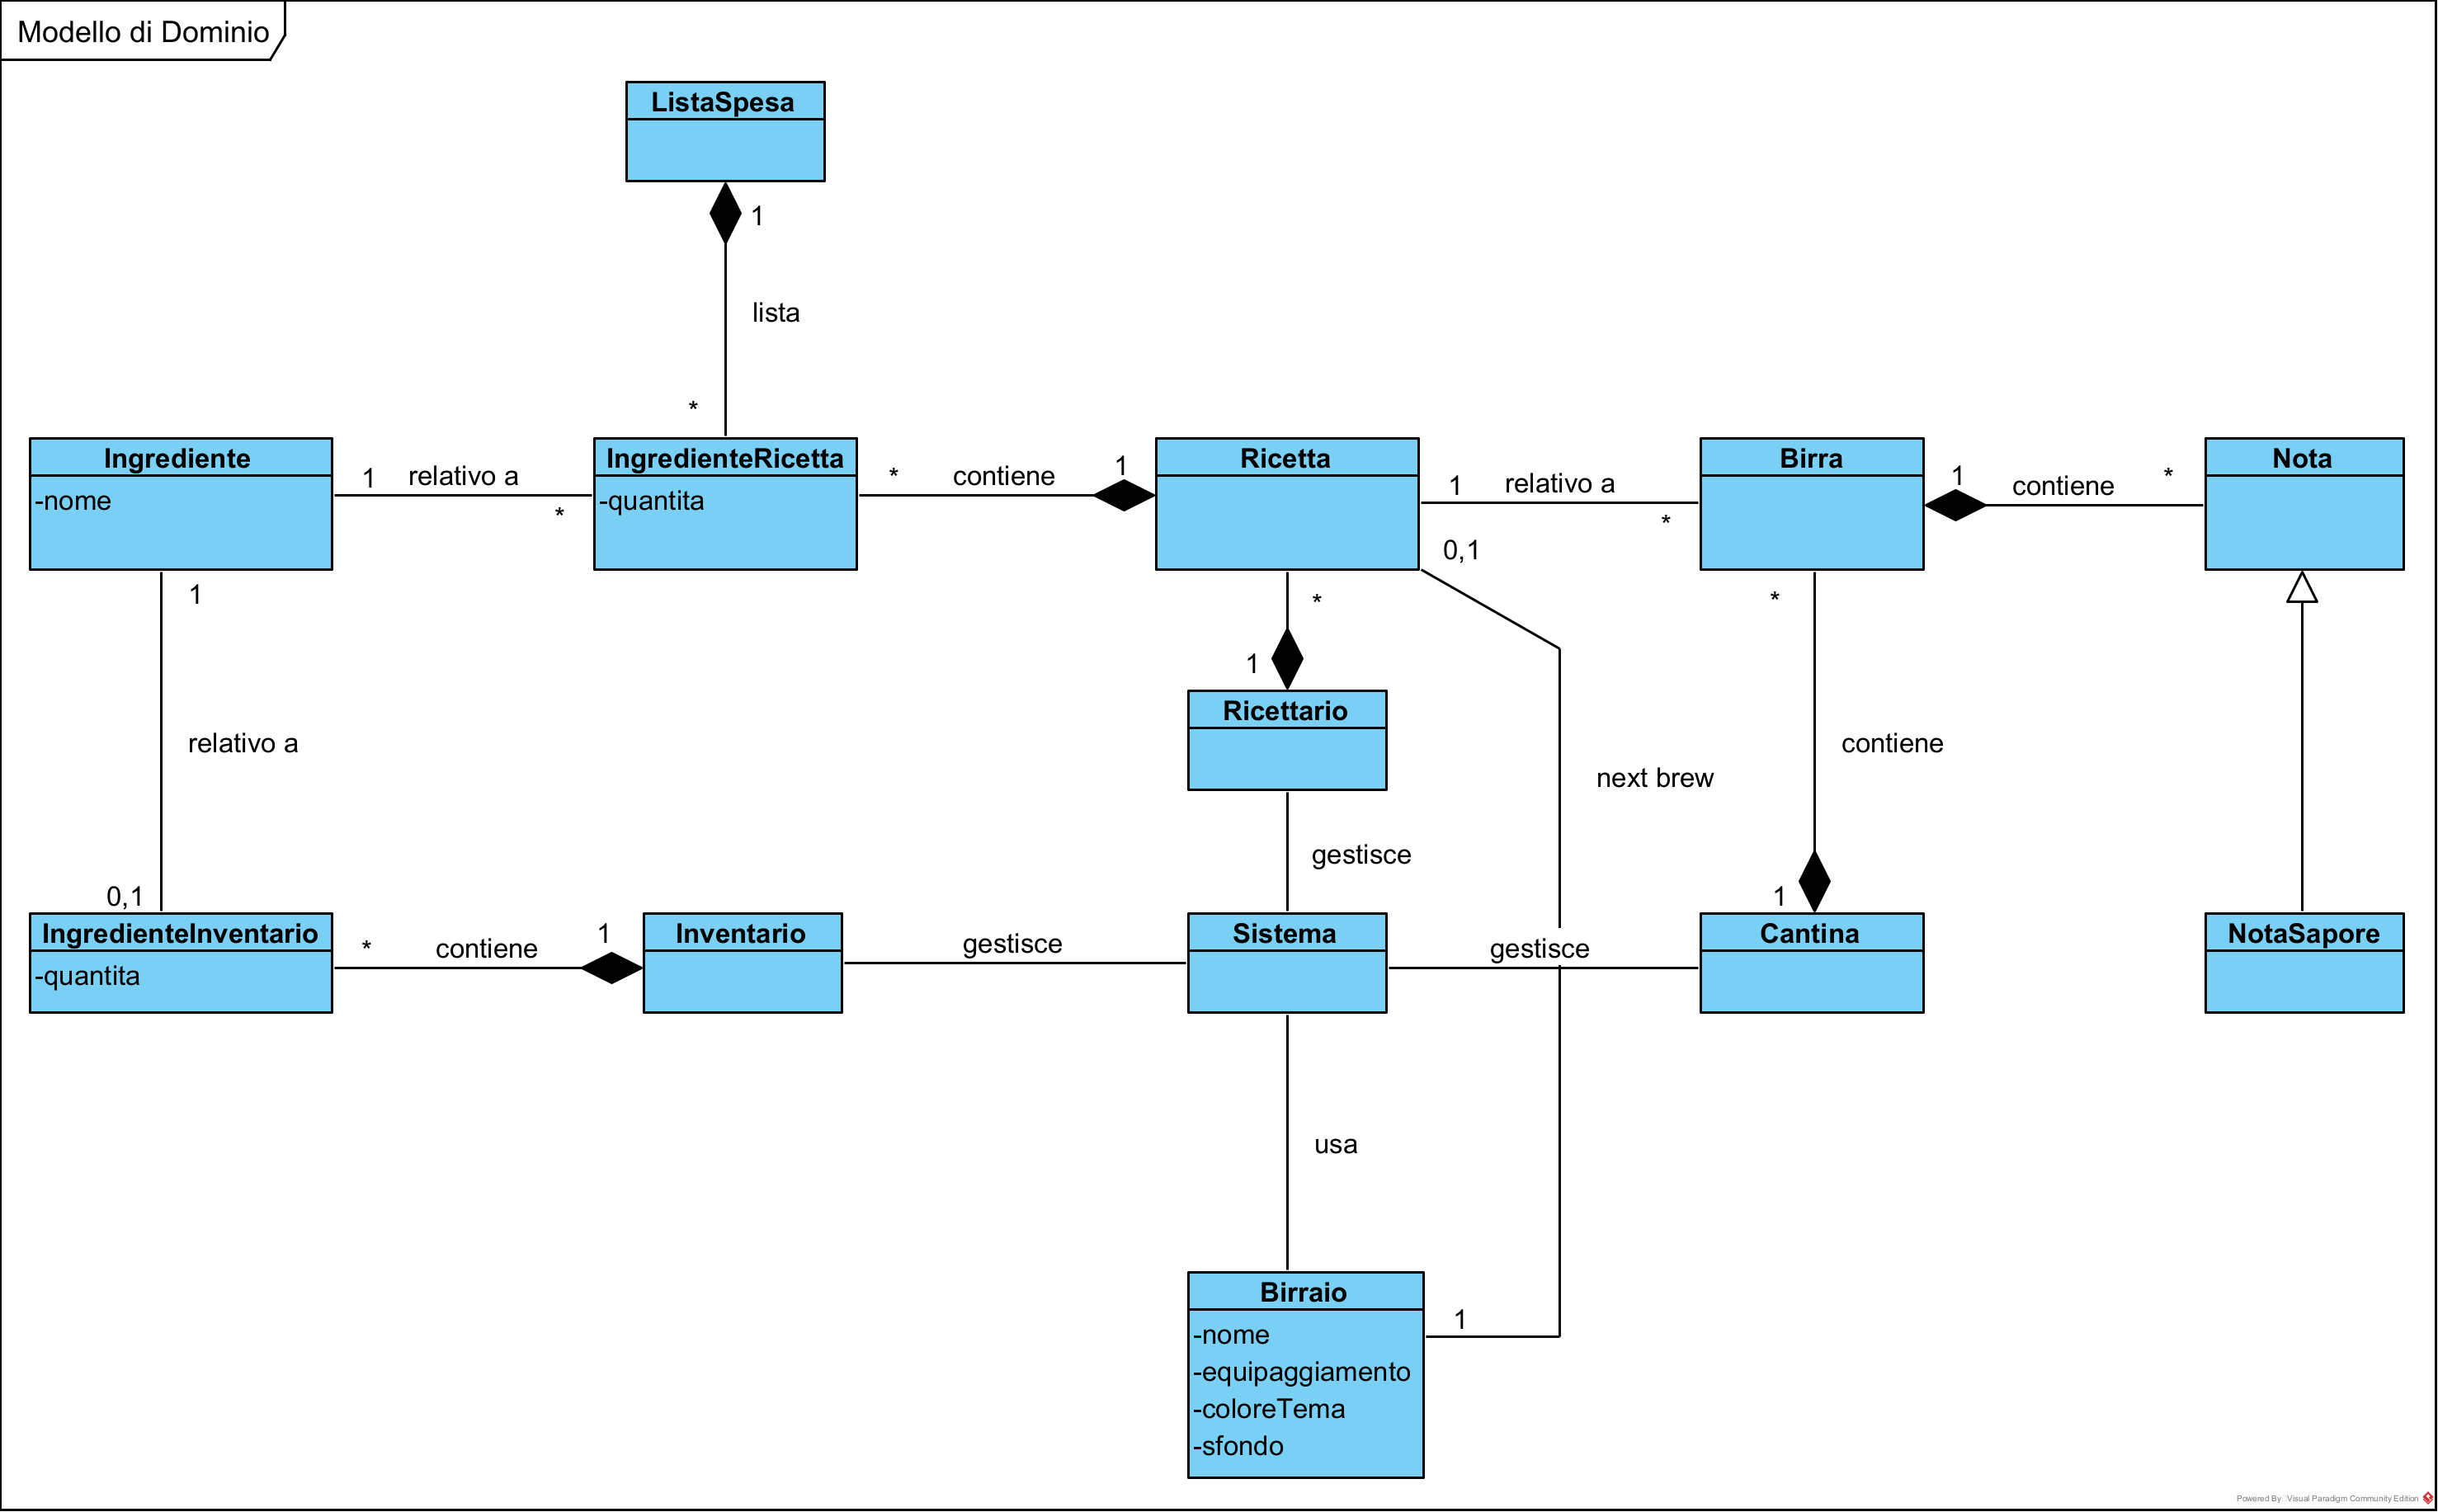
\includegraphics[width=1\linewidth]{image/Modello-di-Dominio.png}
			\caption{Modello di Dominio}\label{fig:Modello-Dominio}
		\end{figure}

	\newpage
	\section{Diagrammi di Sequenza di Sistema}
	Nella prima iterazione sono stati realizzati due diagrammi di sequenza di sistema per rappresentare l'interazione tra l'utente esterno al sistema con l'applicazione.
	I casi scelti sono l'aggiunta di una ricetta nel sistema e la sua modifica.
		\subsection{SSD - aggiungiRicetta}
			E' stato realizzato il diagramma di sequenza di sistema del caso d'suo aggiungiRicetta
			\begin{figure}[!h]
				\centering
				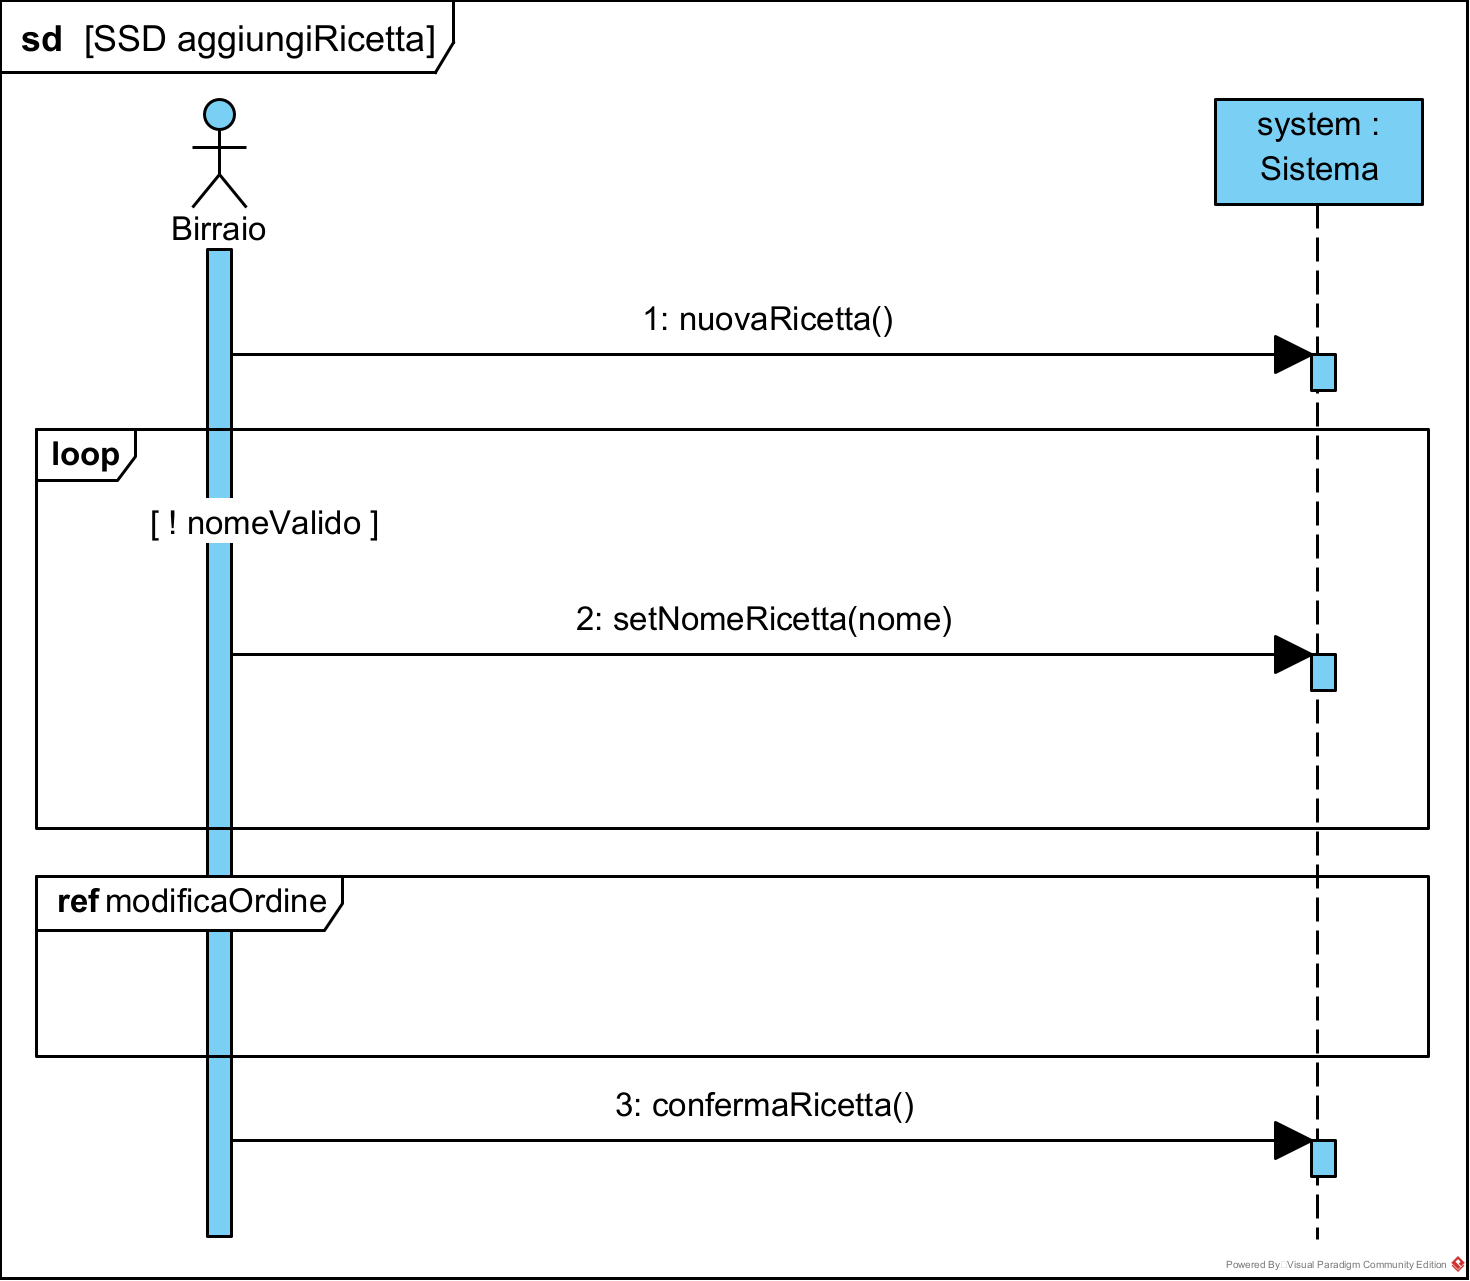
\includegraphics[width=0.8\linewidth]{image/SSD-aggiungiRicetta.png}
				\caption{SSD - aggiungiRicetta}\label{fig:1}
			\end{figure}	
		\newpage	
		\subsection{SSD - modificaRicetta}
			E' stato realizzato il diagramma di sequenza di sistema del caso d'suo modificaRicetta
			\begin{figure}[!h]
				\centering
				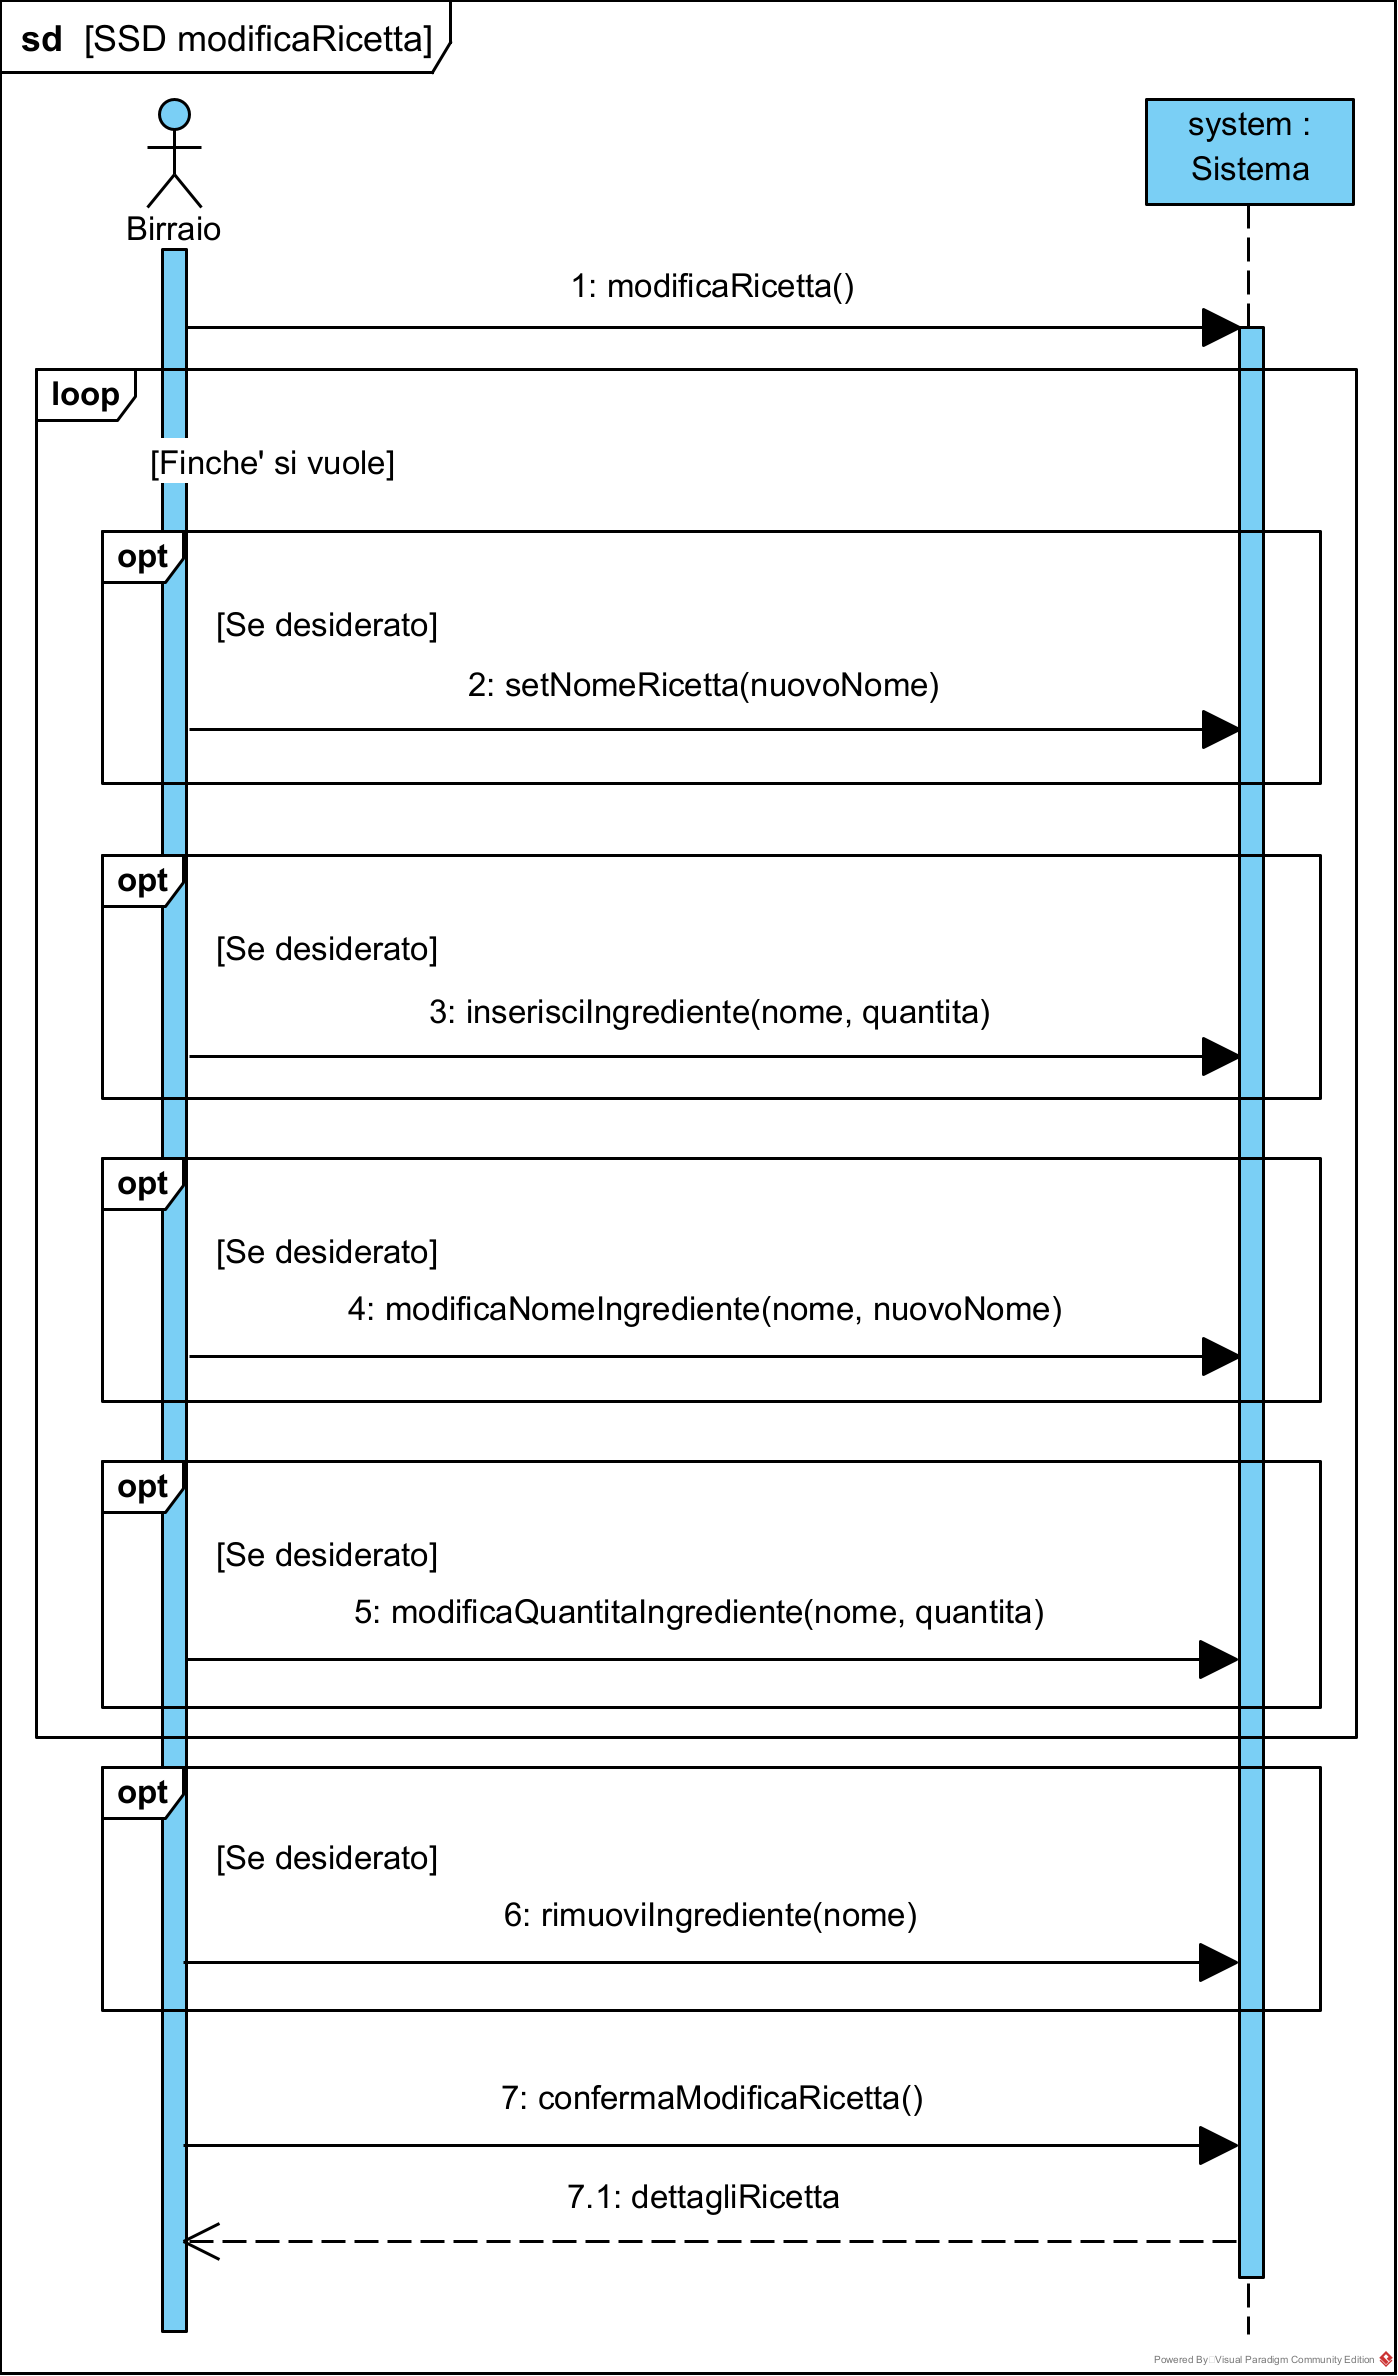
\includegraphics[width=0.7\linewidth]{image/SSD-modificaRicetta.png}
				\caption{SSD - modificaRicetta}\label{fig:1}
			\end{figure}


      \chapter{Progettazione}
     
         \section{Architettura del Software}
Come architettura software è stato scelto di usare un'architettura multi-strato di tipo client-server. Abbiamo suddiviso logicamente le varie funzionalità del software su più strati differenti in comunicazione tra loro. Gli strati individuati sono UI, Application, Domain, Technical Services.
		\begin{figure}[!h]
			\centering
			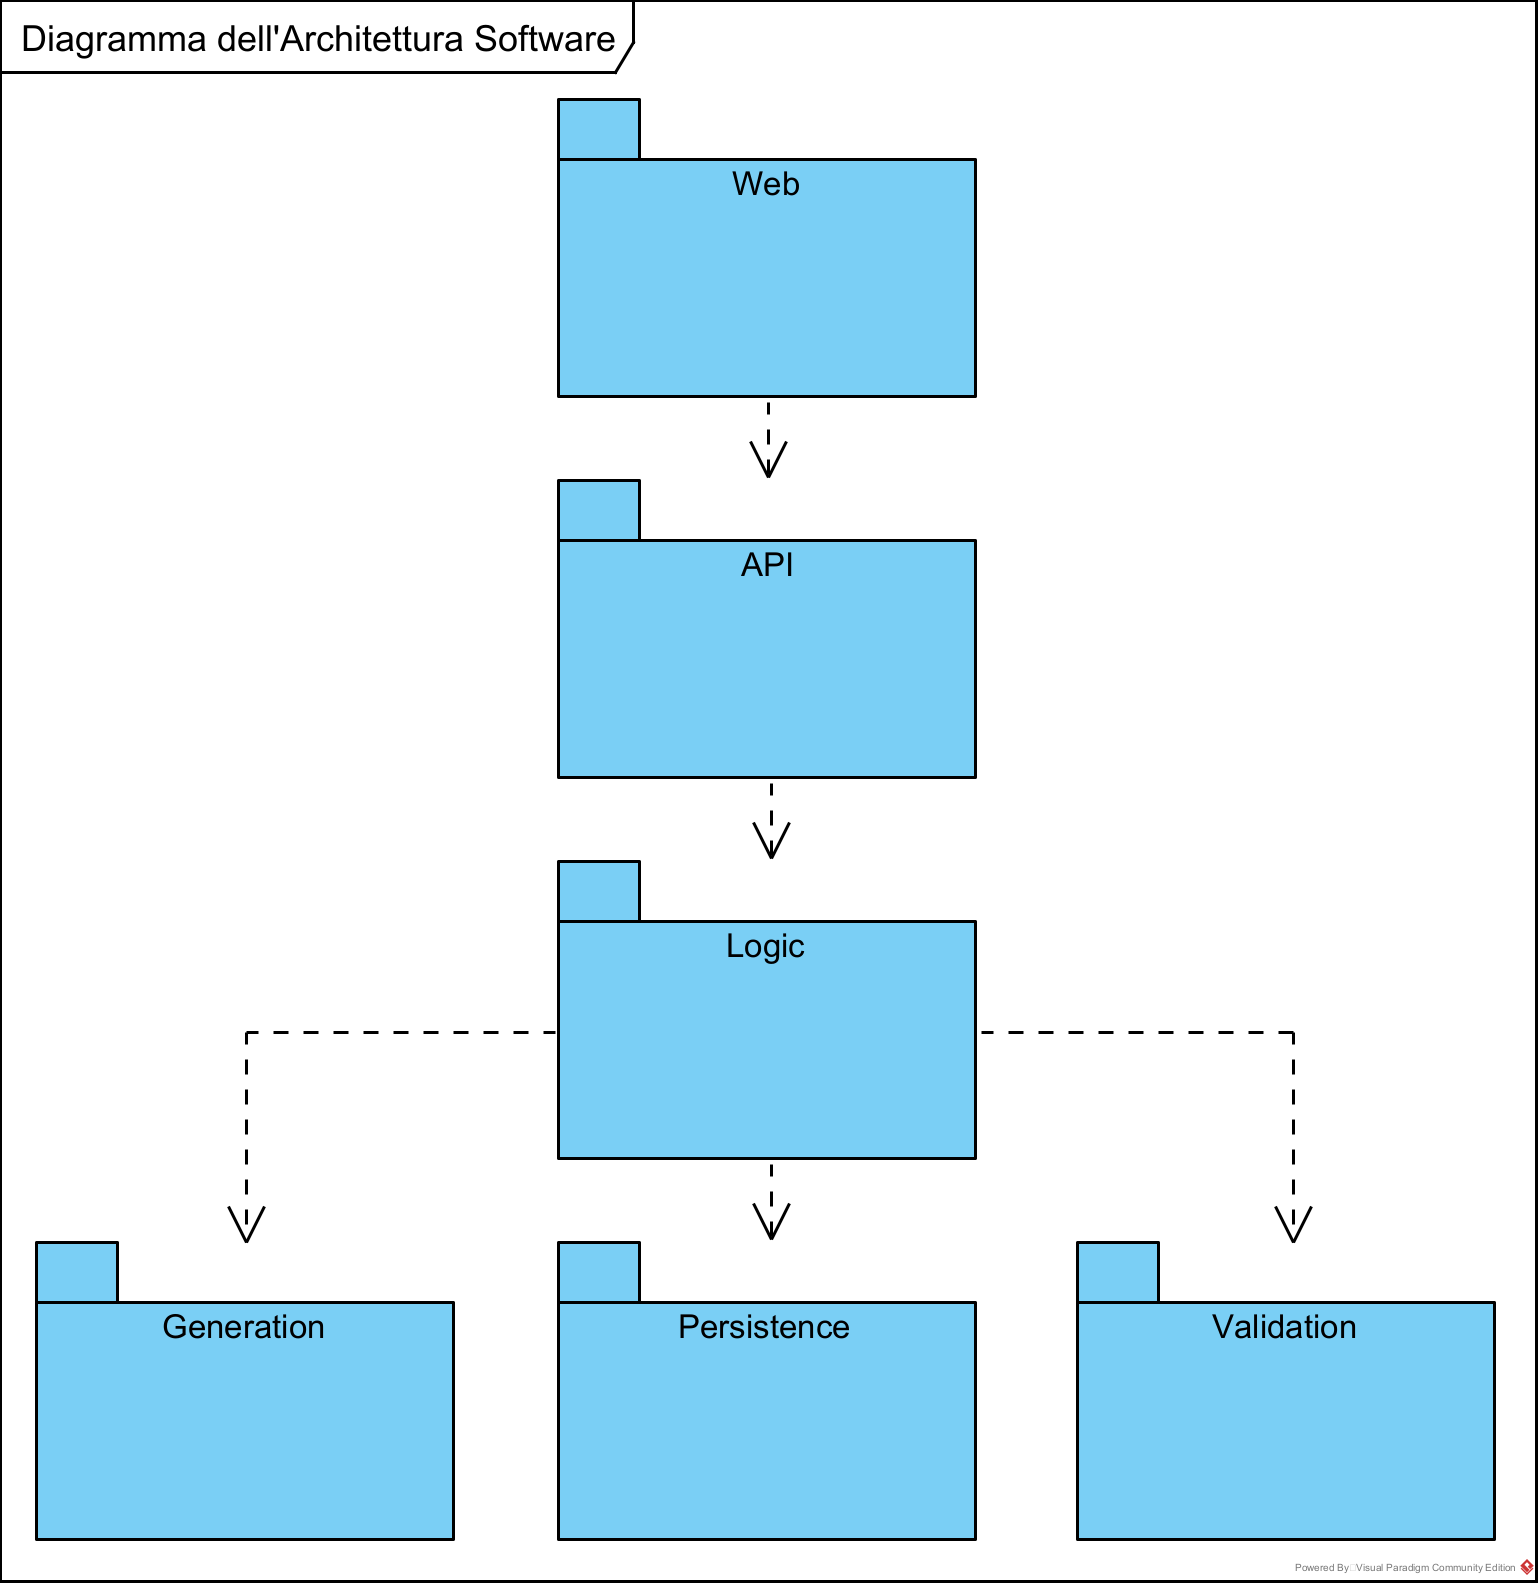
\includegraphics[width=0.5\linewidth]{image/Diagramma-dell'Architettura-Software.png}
			\caption{Diagramma dell'Architettura Software}\label{fig:Diagramma-dell'Architettura-Software.}
		\end{figure}         
\newpage
		\subsection{Design Principles}
			\subsubsection{Interface Segregation Principle}		
Applicando questo principio di sviluppo ci siamo sincerati di aver suddiviso il più possibile le responsabilità e le attività svolte dai singoli controller.
			\subsubsection{Single Responsibility Principle}
Le classi Handler per la validazione dei dati e le classi che compongono il package Generation aggiungono una e una sola responsabilita' al contesto in cui sono utilizzate.
Per esempio si e' scelto appositamente di spezzettare il piu' possibile la catena per la generazione degli ID separando la classe che usa una funzione di Hashing da quella che genera un Seed randomico da usare insieme al Seed di input.
Altro esempio e' il fatto che ogni Handler si occupa di un punto specifico a atomico della validazione dell'input.
			\subsubsection{Open–closed principle}
Le classi del package Generation permettono di aggiungere pezzi di computazione senza modificare la classi da cui derivano.

         
         \section{Diagramma delle Classi di Progettazione}
Durante le iterazioni sono stati creati/aggiornati i diagrammi delle classi, che descrivono gli aspetti statici del sistema, classi, la loro struttura e le relazioni con altre classi.
Di seguito vengono riportati tutti i diagrammi di classi realizzati, suddivisi per Package. Nello specifico, abbiamo il diagramma delle classi per il package Api, Logic, Persistence, Validation e Generation.

		\subsection{Diagramma delle Classi Api}
			\begin{figure}[!h]
				\centering
				\includegraphics[width=01\linewidth]{image/Diagramma-delle-Classi-Api.png}
				\caption{Diagramma delle Classi  Api}\label{fig:1}
			\end{figure}         		
\newpage			
  		\subsection{Diagramma delle Classi Logic}
			\begin{figure}[!h]
				\centering
				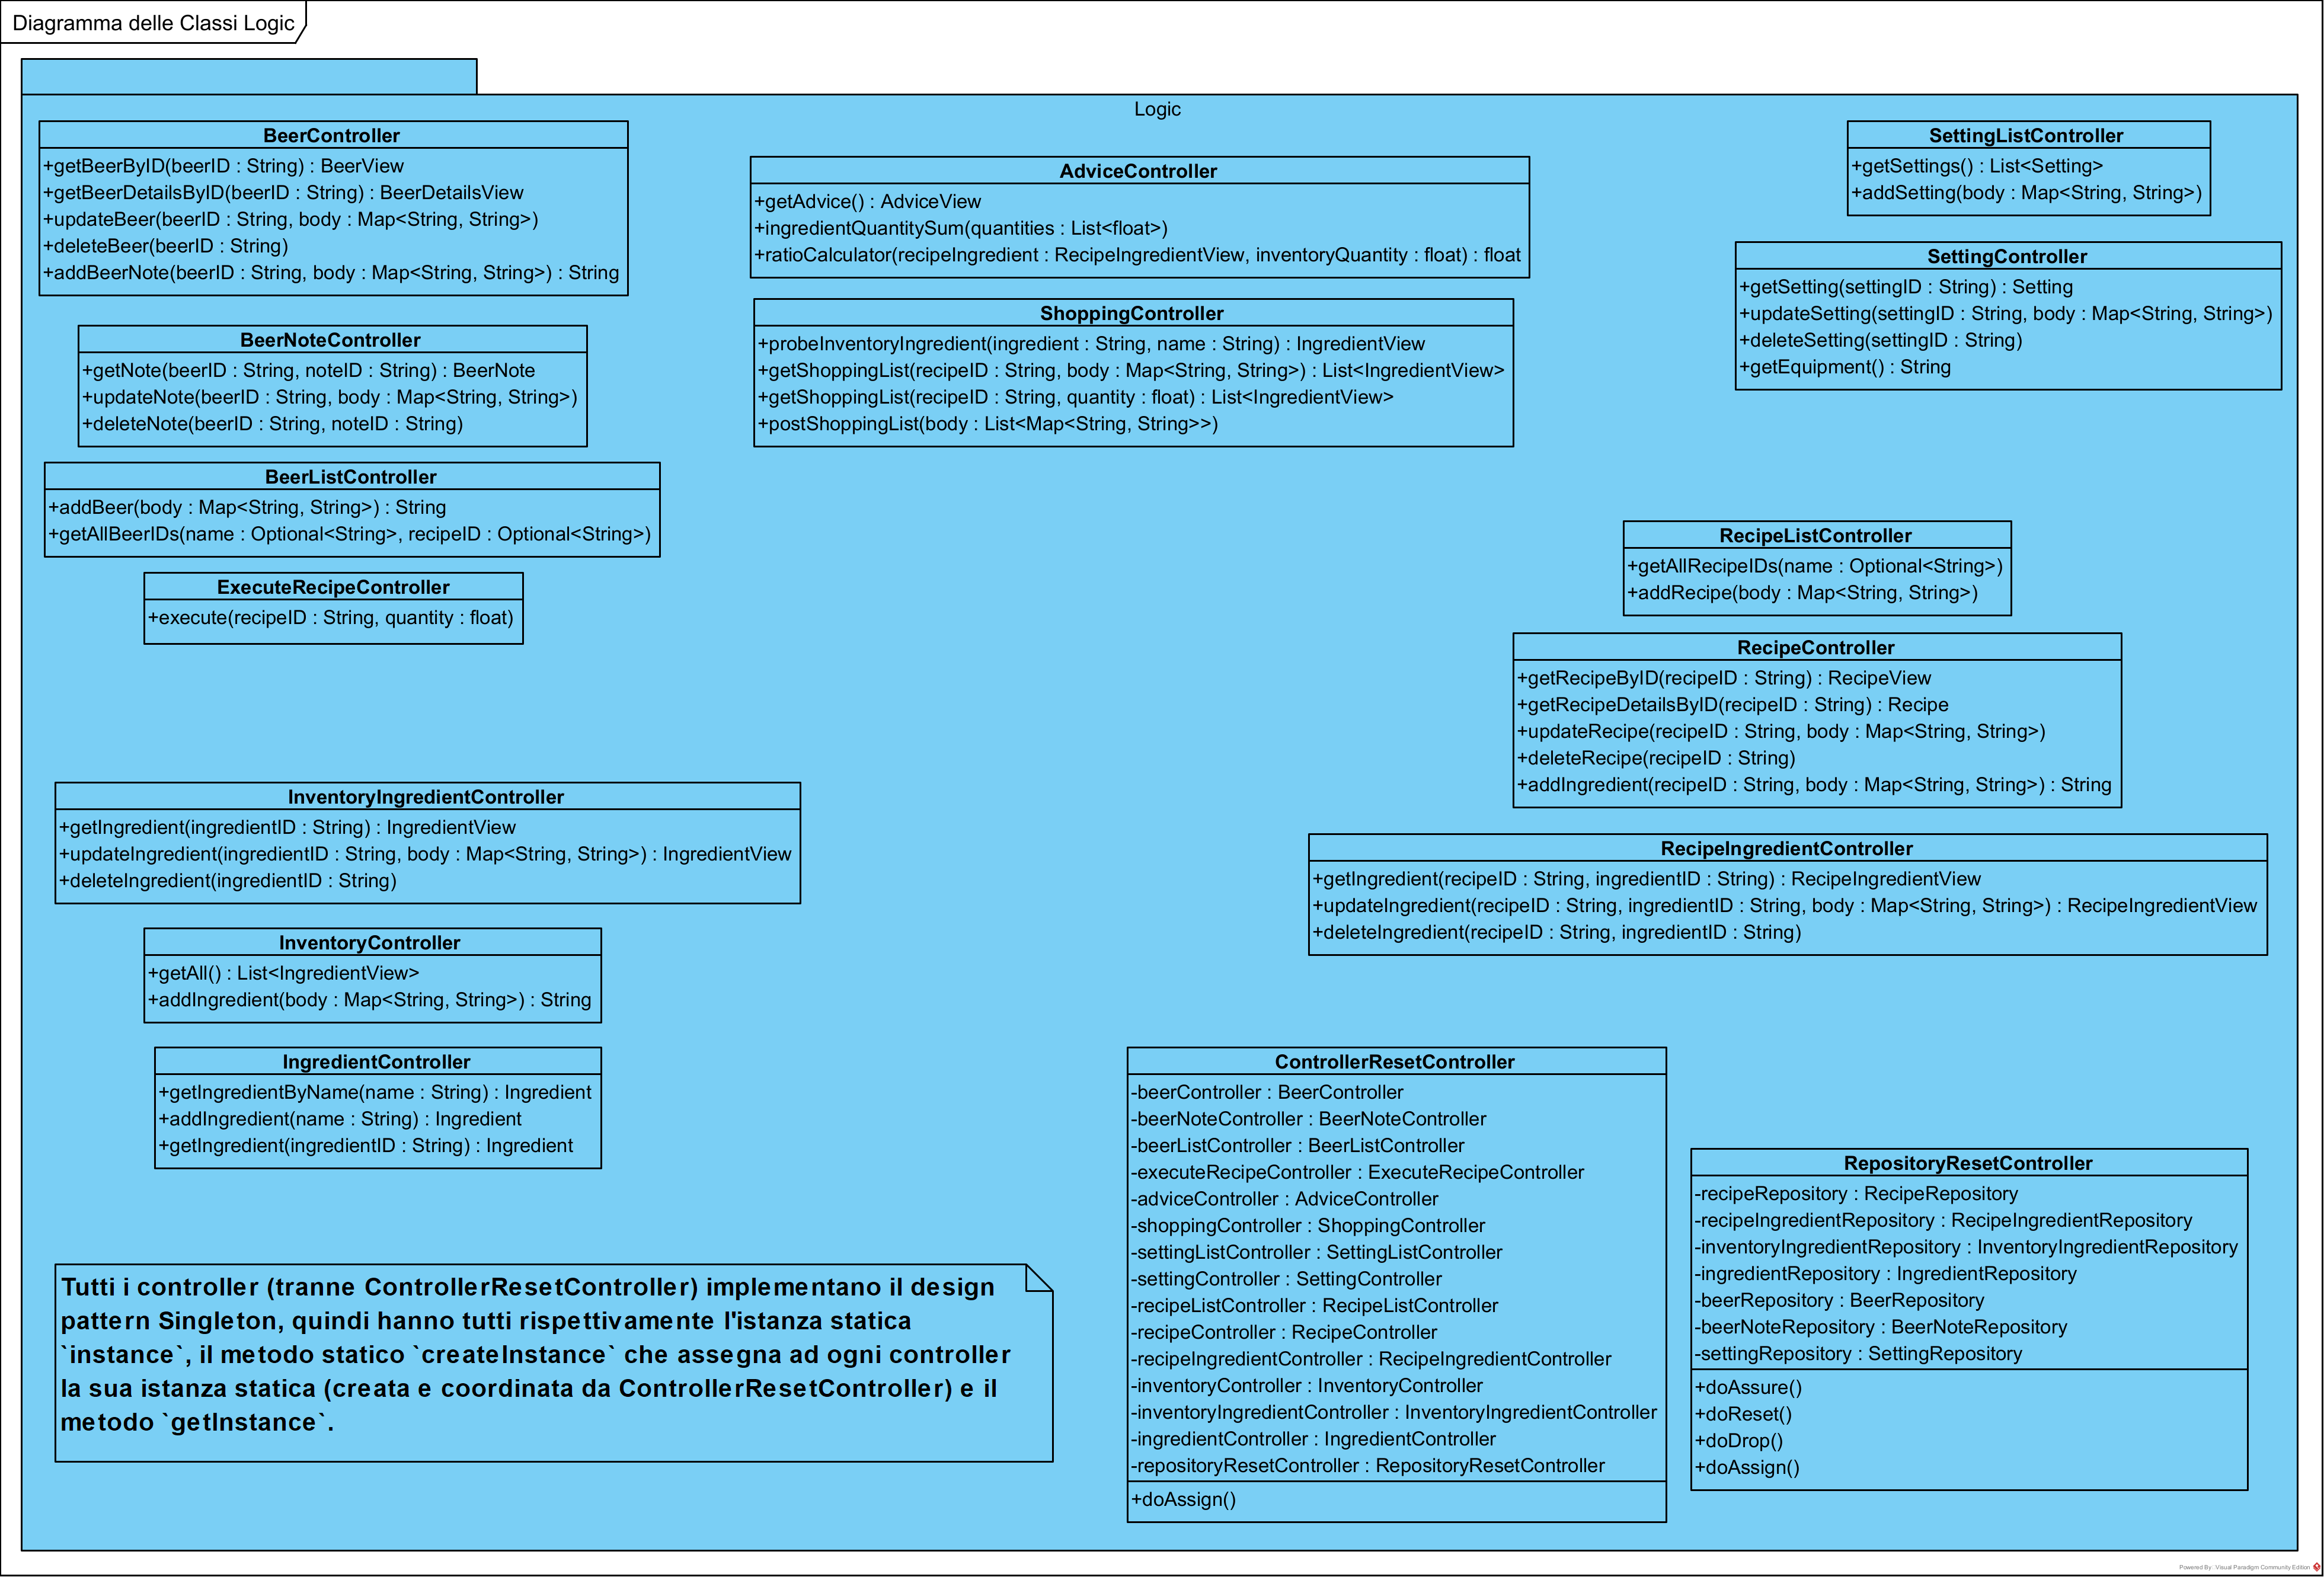
\includegraphics[width=0.9\linewidth]{image/Diagramma-delle-Classi-Logic.png}
				\caption{Diagramma delle Classi Logic  }\label{fig:1}
			\end{figure}  
			
		\subsection{Diagramma delle Classi Validation}
			\begin{figure}[!h]
				\centering
				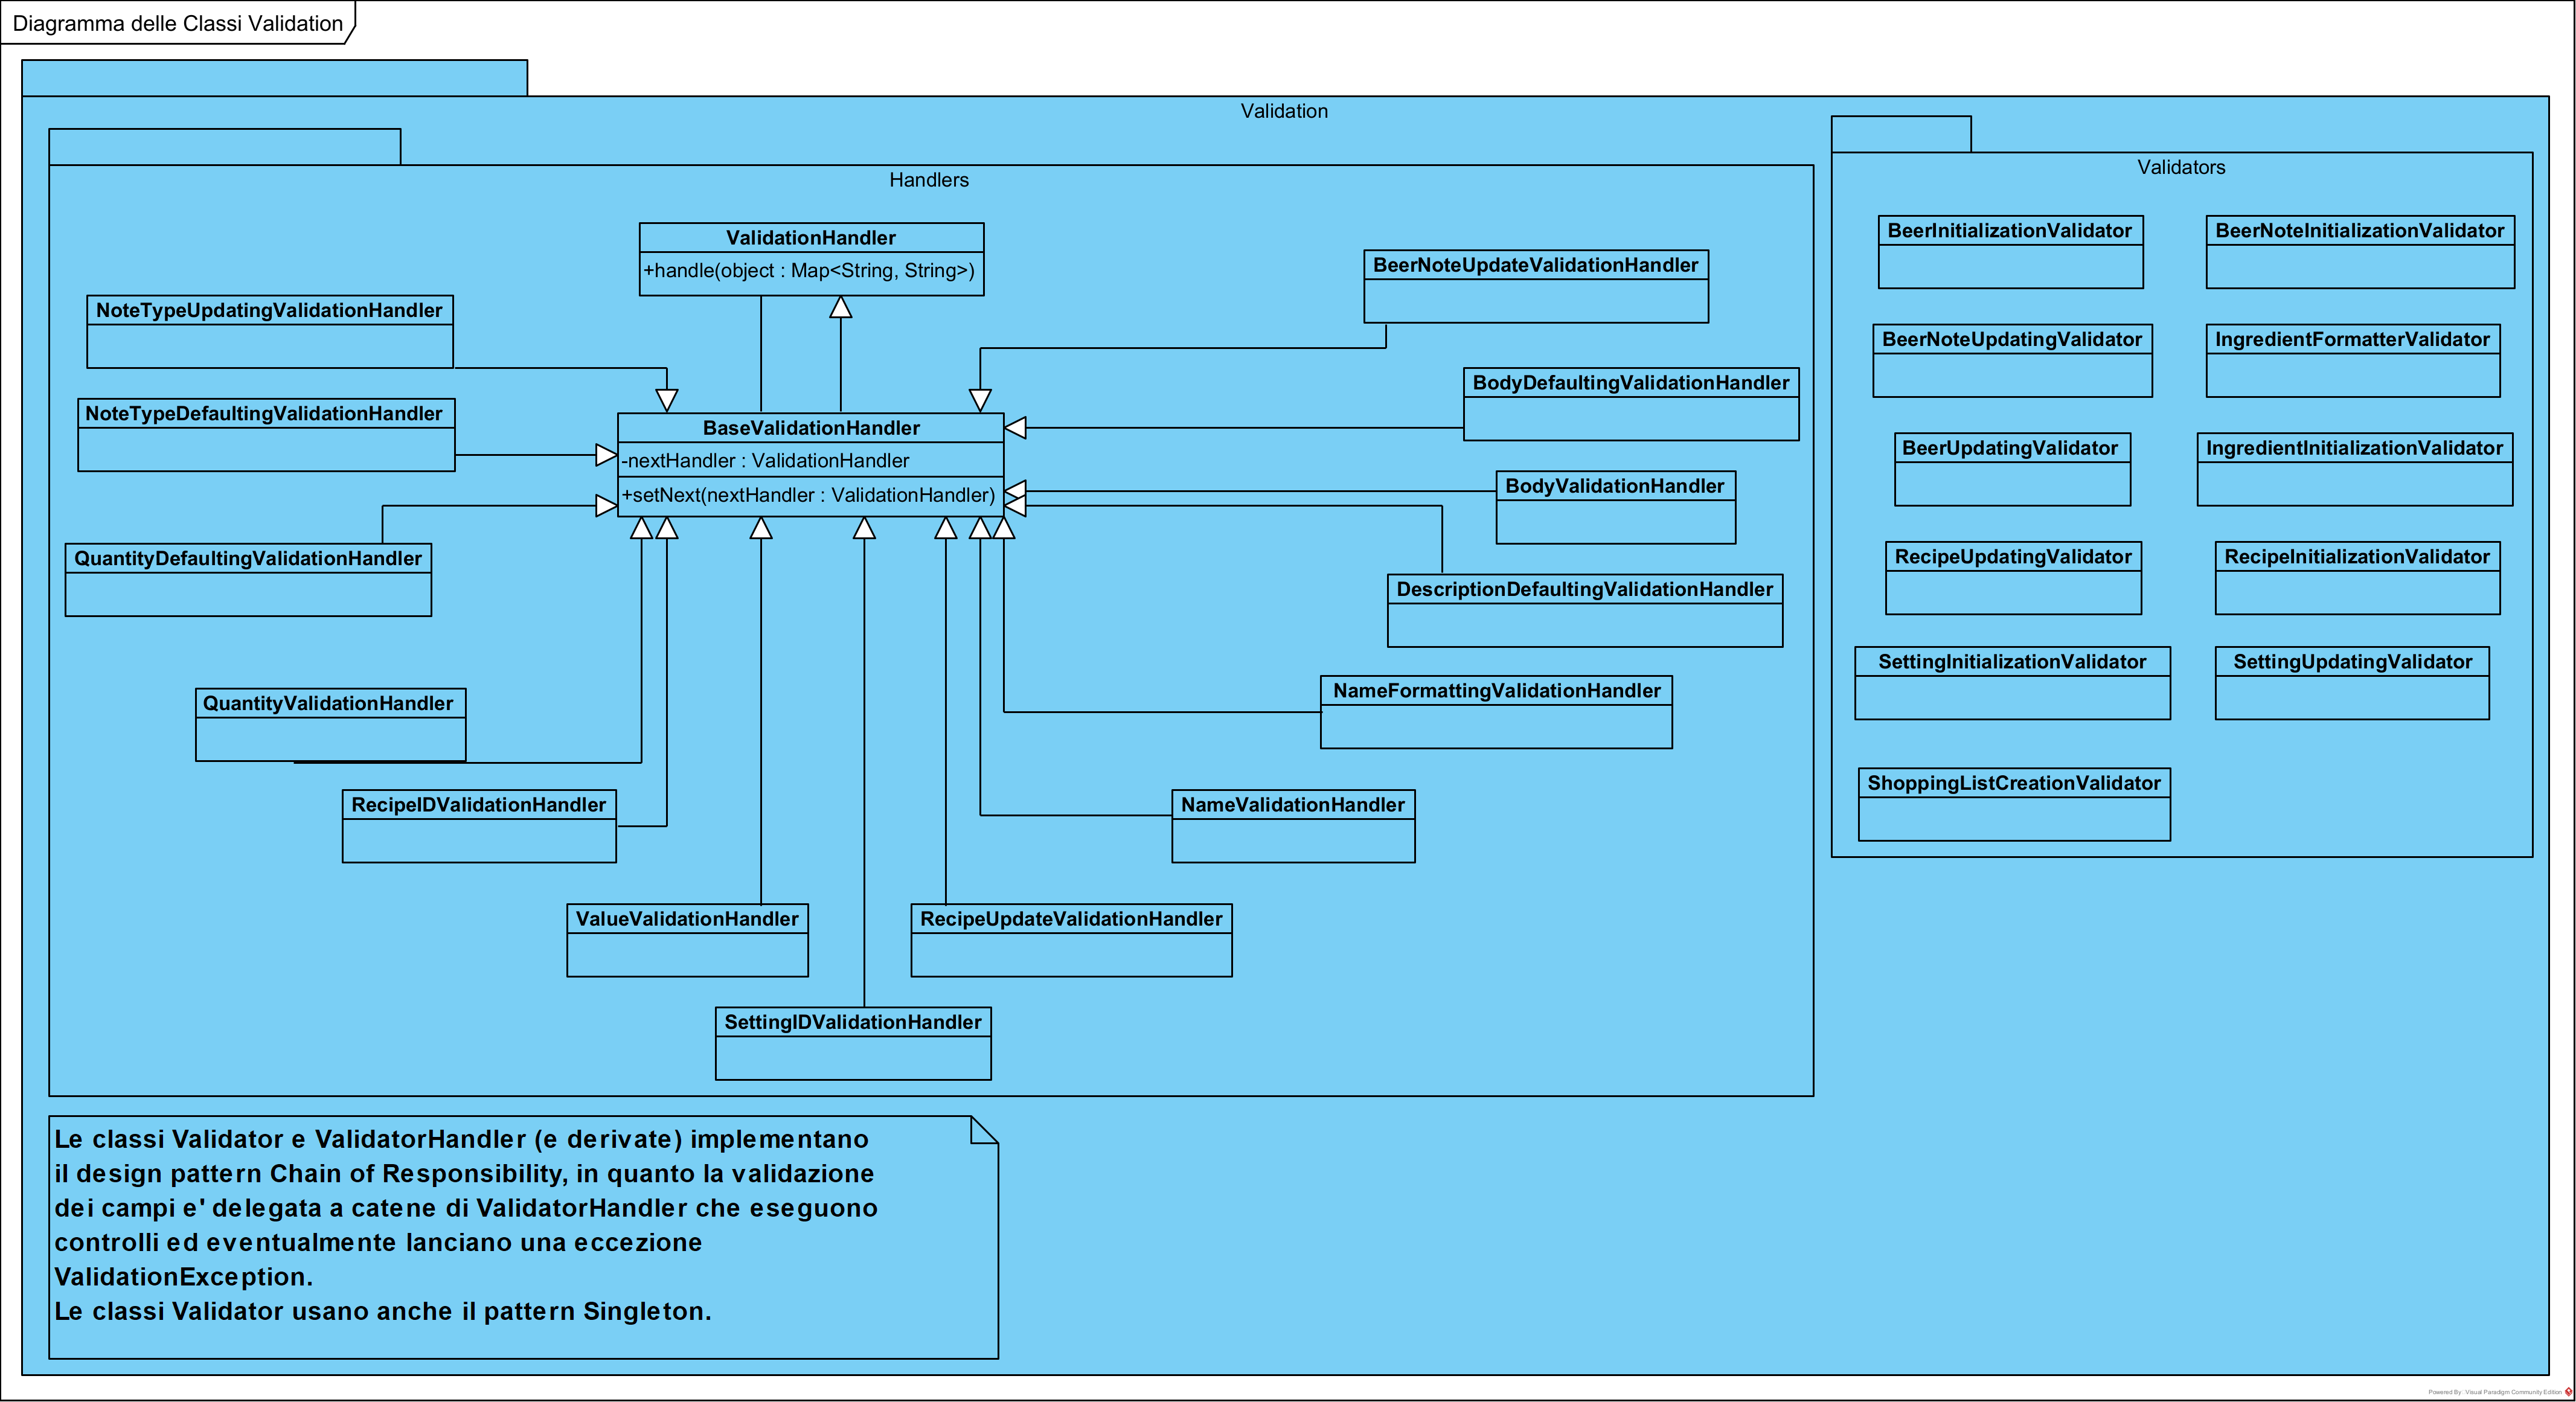
\includegraphics[width=0.9\linewidth]{image/Diagramma-delle-Classi-Validation.png}
				\caption{Diagramma delle Classi Validation}\label{fig:1}
			\end{figure}           
\newpage
		\subsection{Diagramma delle Classi Persistence}
			\begin{figure}[!h]
				\centering
				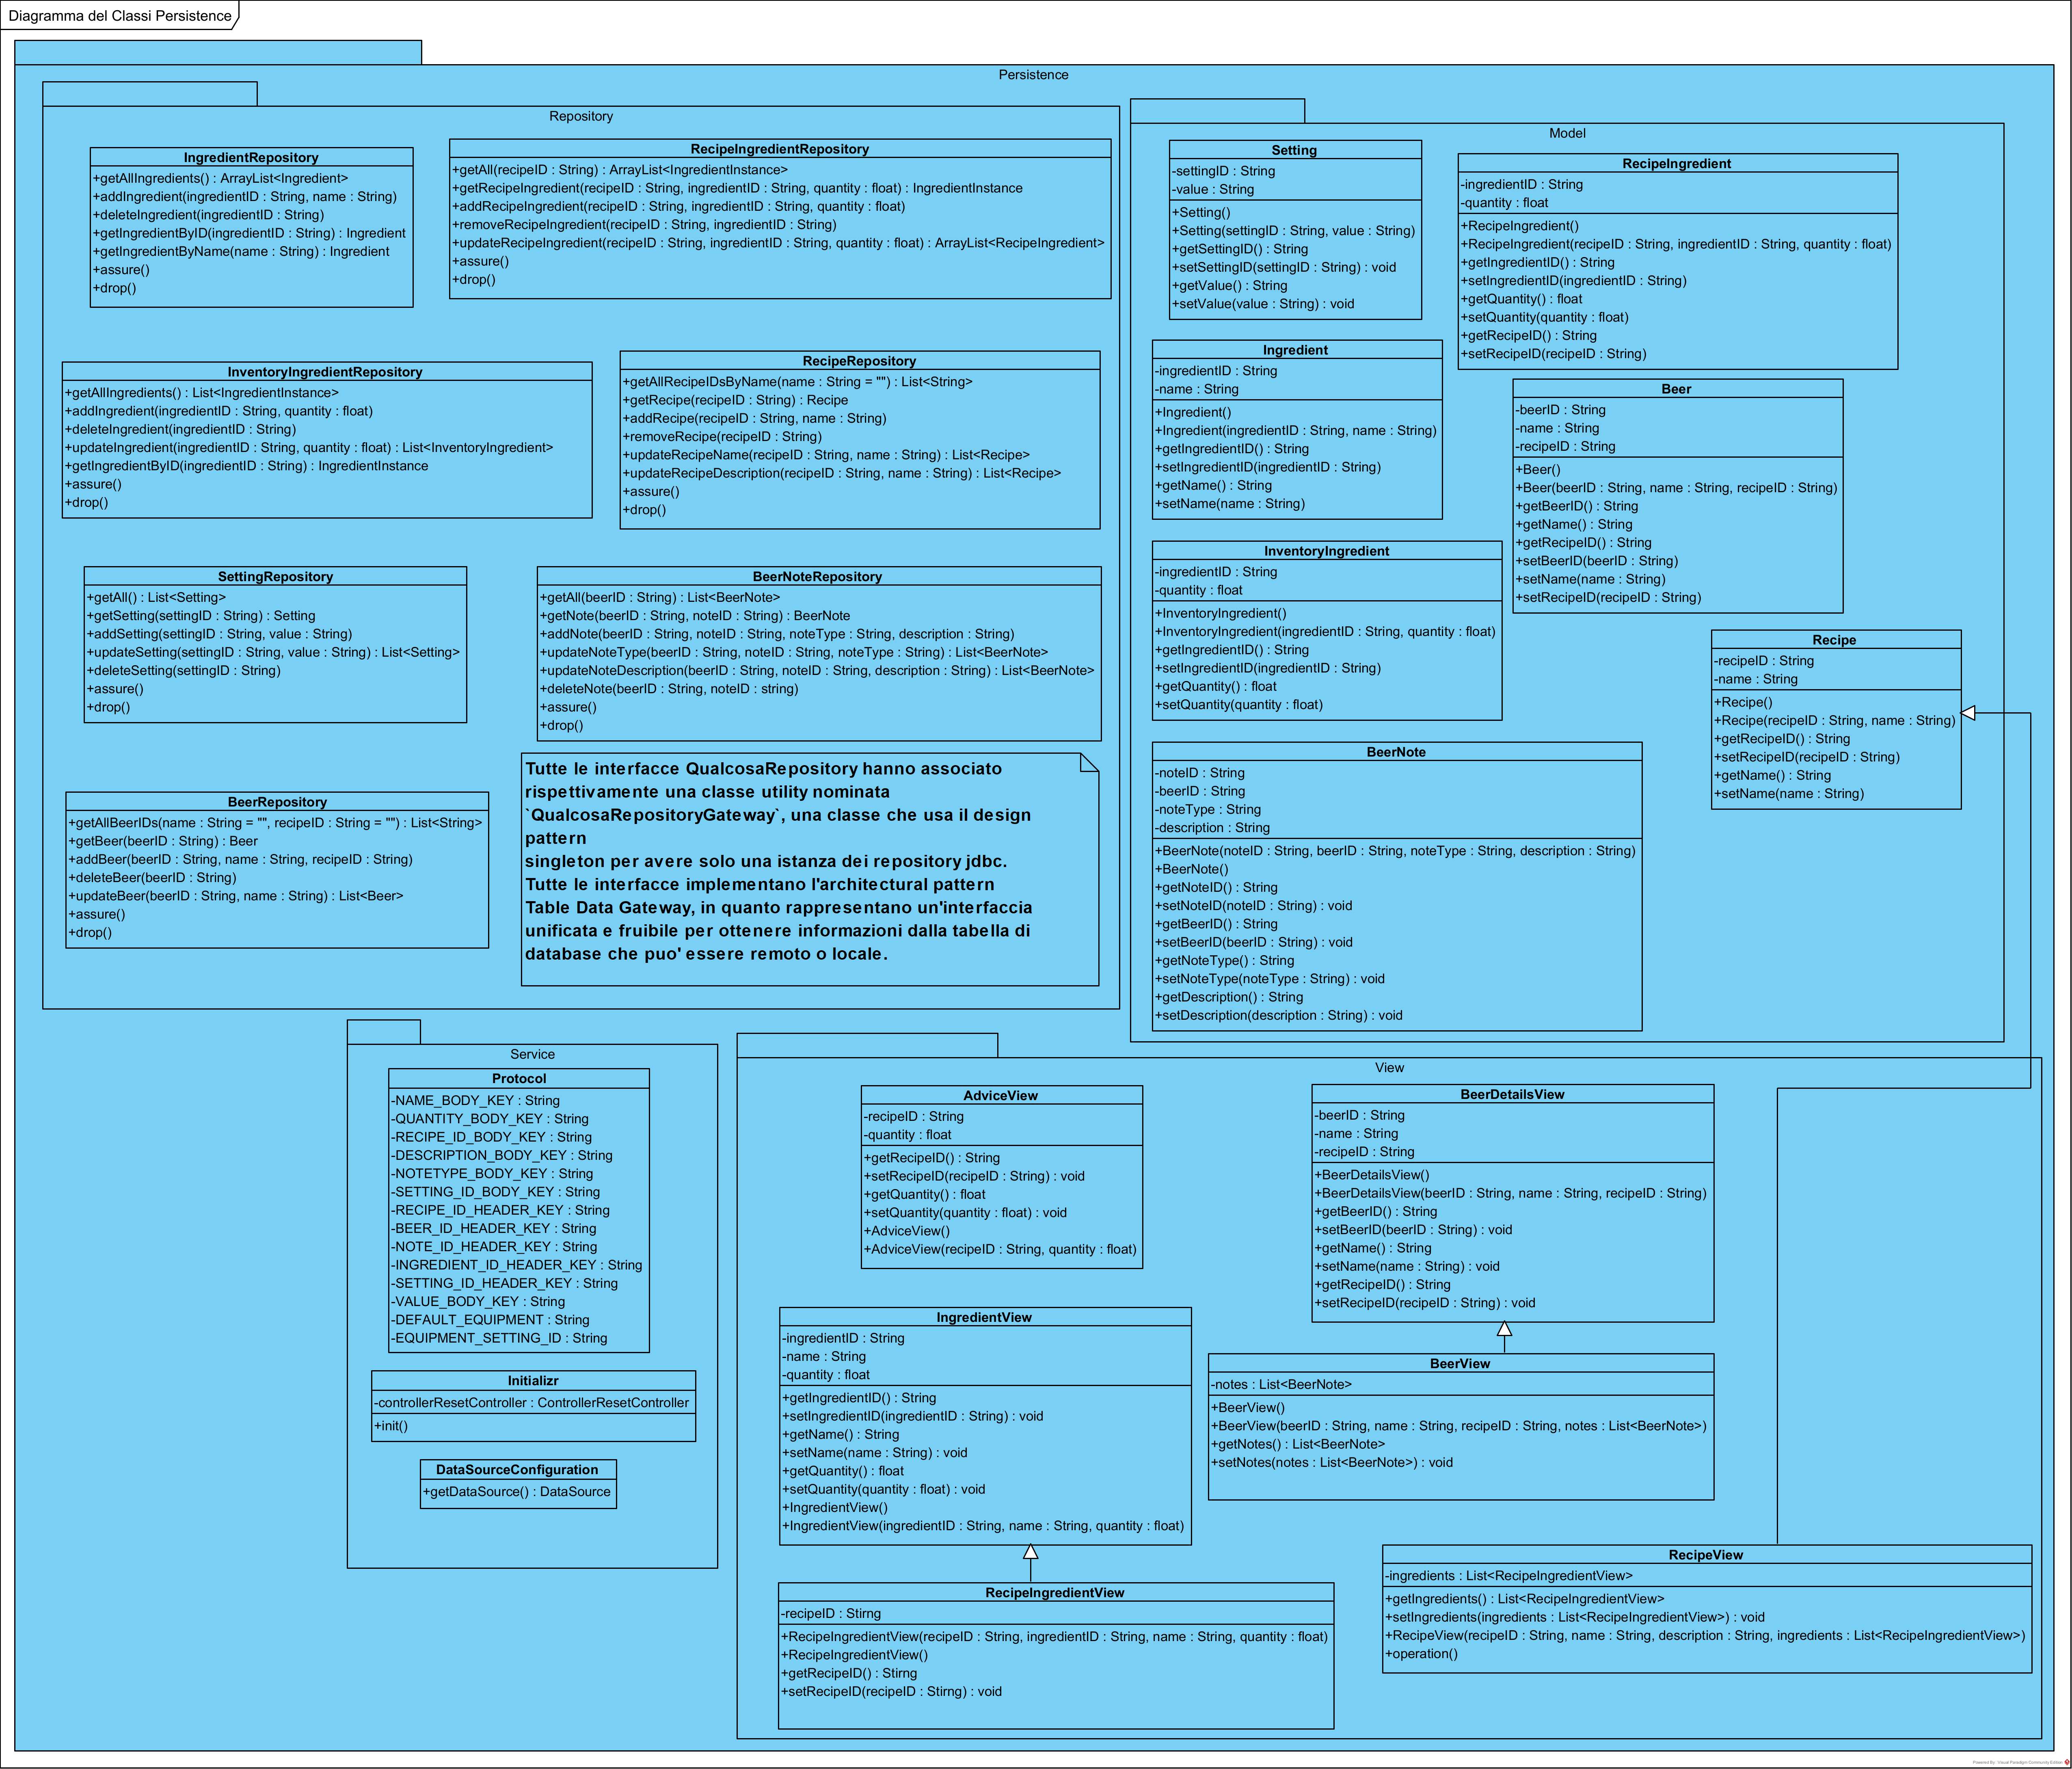
\includegraphics[width=01\linewidth]{image/Diagramma-delle-Classi-Persistence.png}
				\caption{Diagramma delle Classi Persistence}\label{fig:1}
			\end{figure}             

		\subsection{Diagramma delle Classi Generation}
			\begin{figure}[!h]
				\centering
				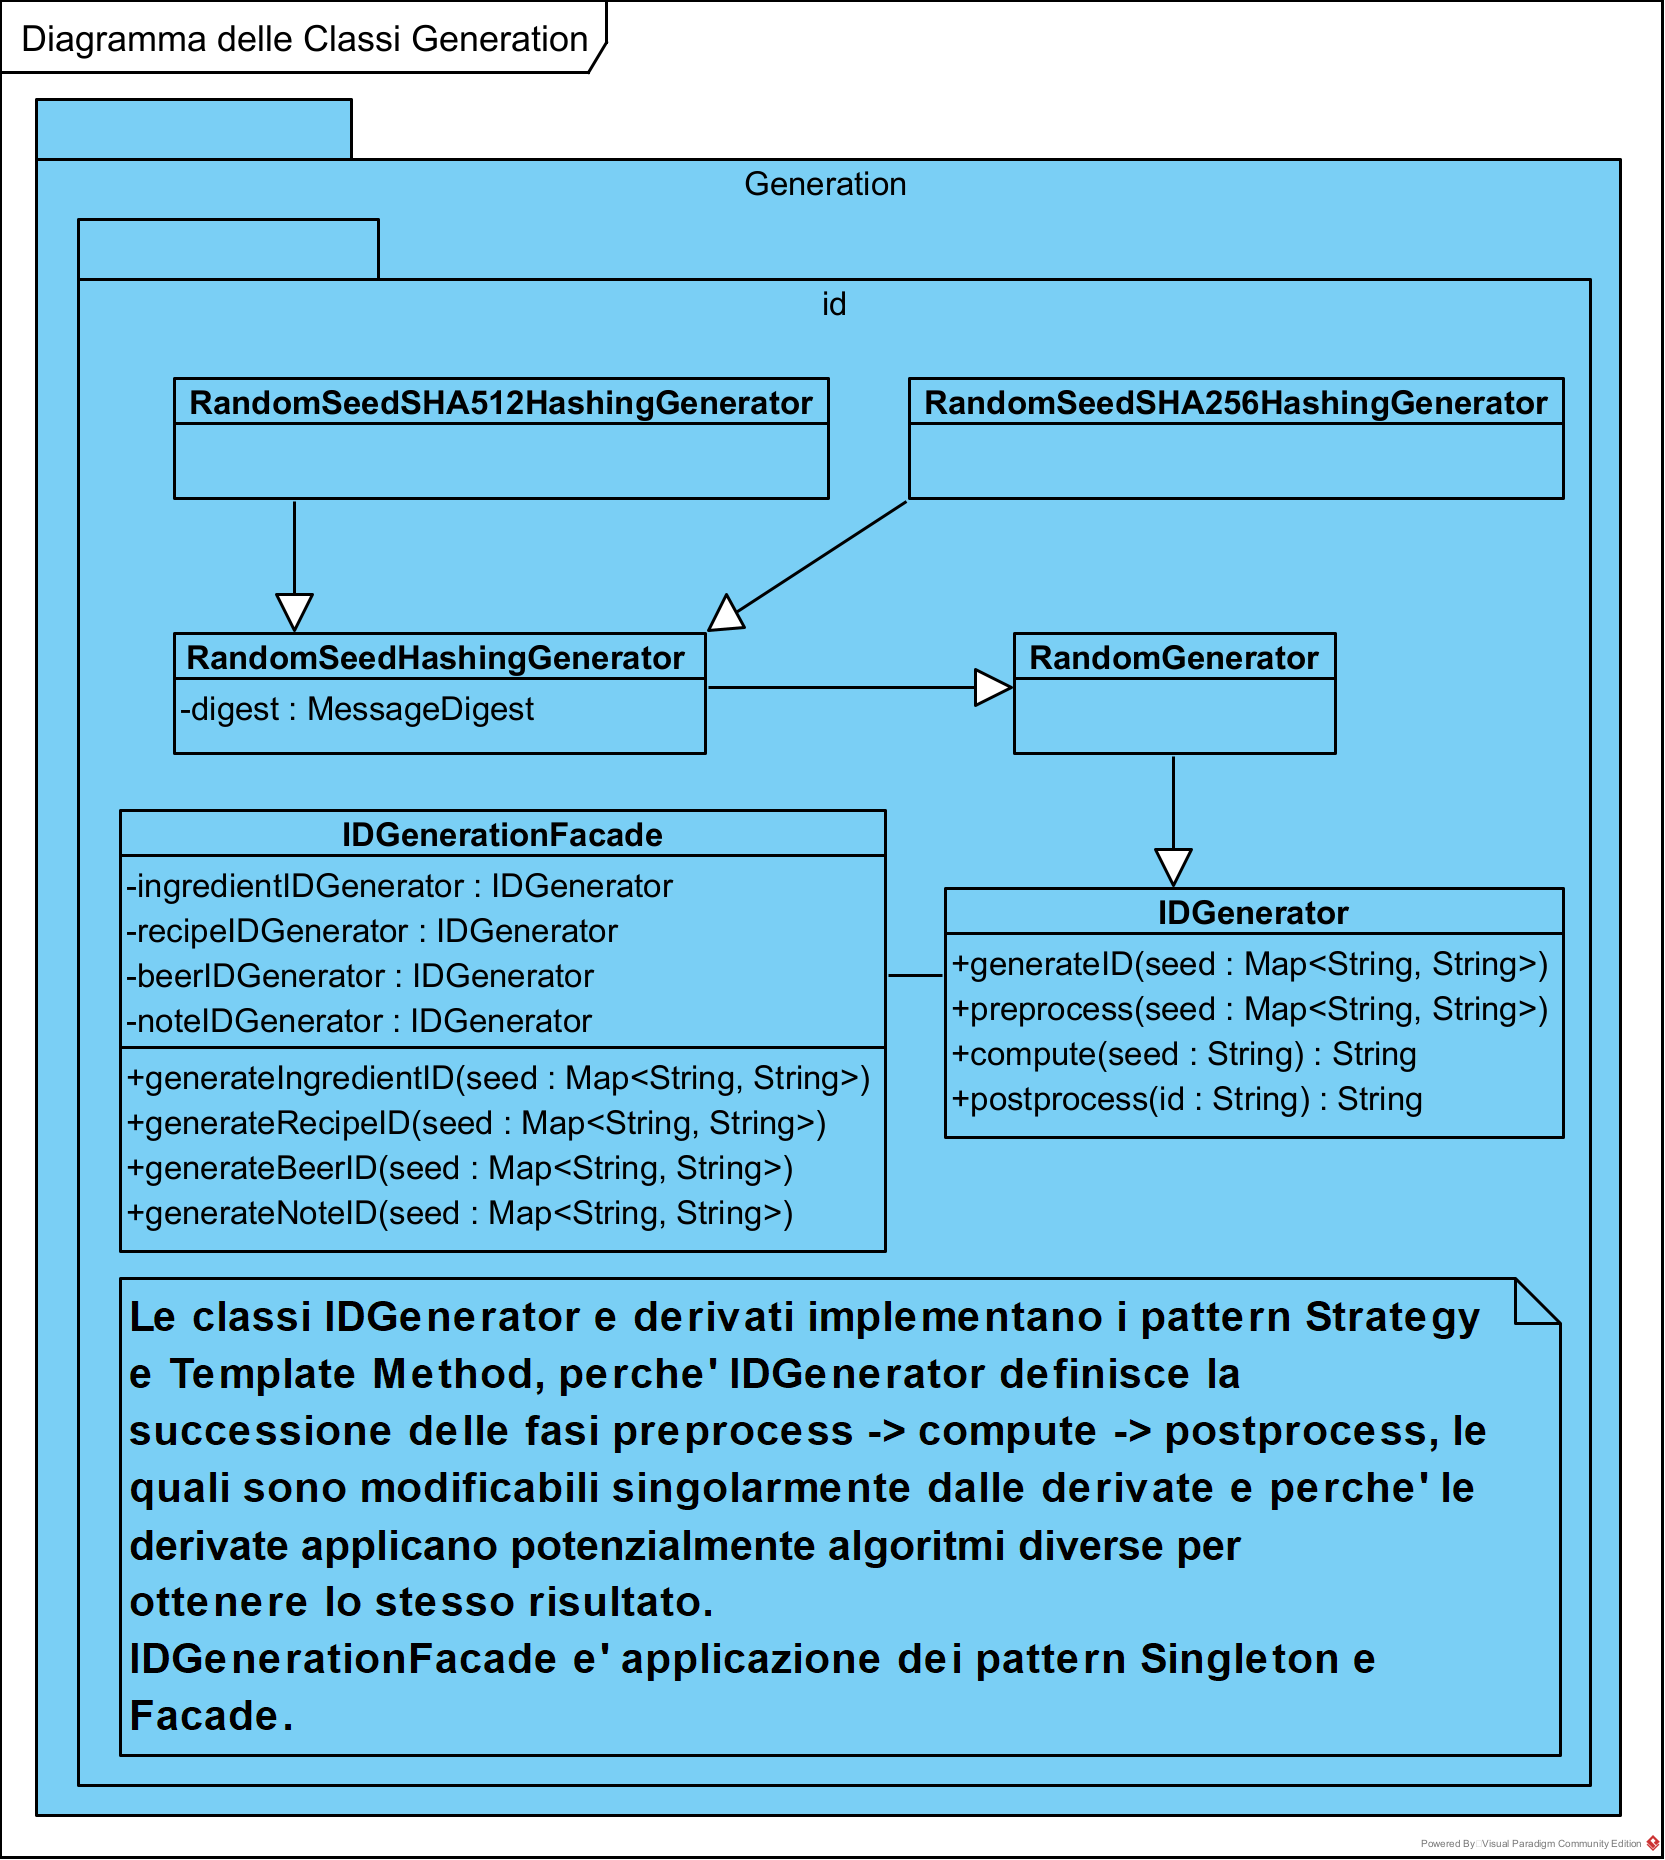
\includegraphics[width=0.3\linewidth]{image/Diagramma-delle-Classi-Generation.png}
				\caption{Diagramma delle Classi Generation}\label{fig:1}
			\end{figure}  
			
    \newpage
      	\section{Diagrammi di Sequenza} 
	Nella prima iterazione abbiamo realizatto due diagrammi di sequenza per illustrare le interazioni tra gli oggetti del sistema.
		\subsection{SD - modificaQuantitaIngrediente}
			E' stato realizzato il diagramma di sequenza di modificaQuantitaIngrediente appartenente al caso d'suo modificaRicetta (figura \ref{fig:SD-modificaQuantitaIngrediente}).
			Si ha l'interazione tra l'oggetto Ricetta e IngredienteRicetta.
			\begin{figure}[!h]
				\centering
				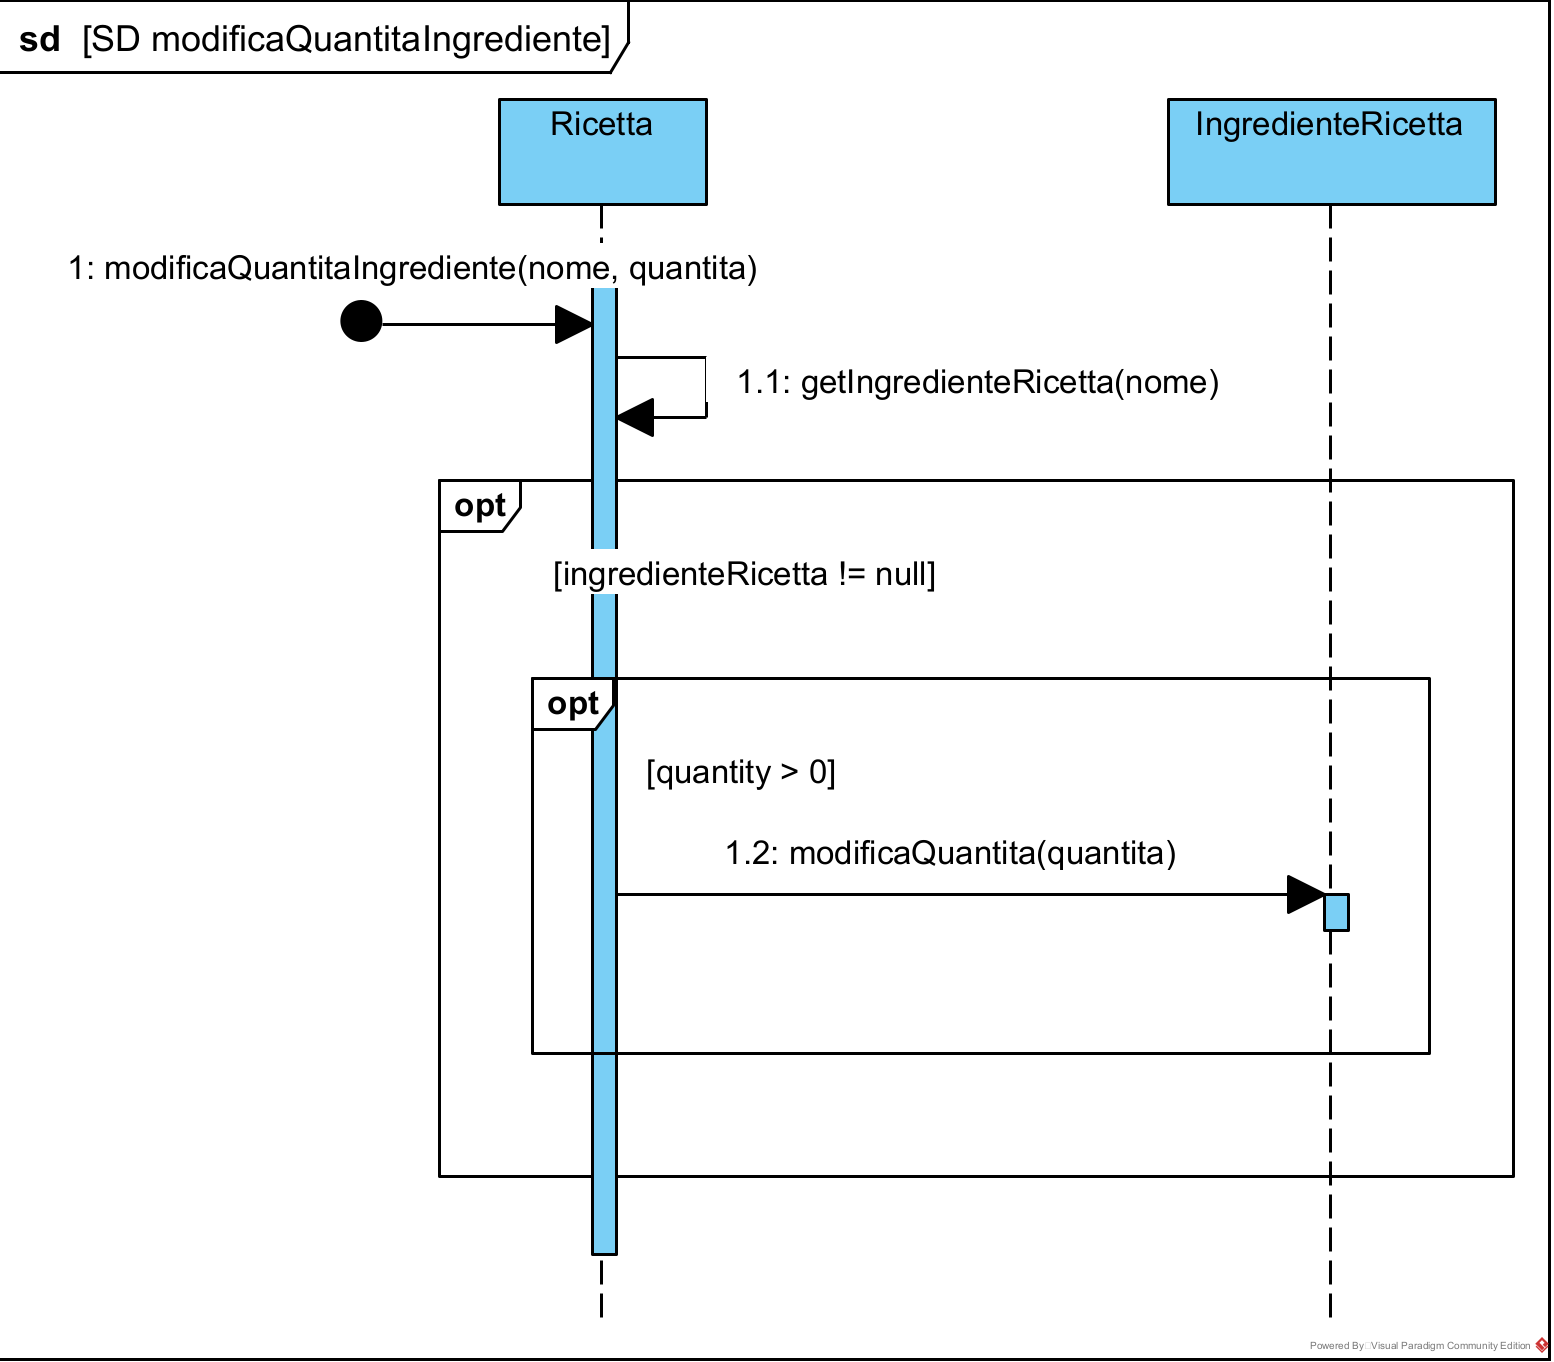
\includegraphics[width=0.7\linewidth]{image/SD-modificaQuantitaIngrediente.png}
				\caption{SD - modificaQuantitaIngrediente}\label{fig:SD-modificaQuantitaIngrediente}
			\end{figure}	
		\newpage	
		\subsection{SD - modificaNomeIngrediente}
			E' stato realizzato il diagramma di sequenza di modificaNomeIngrediente appartenente al caso d'suo modificaRicetta (figura \ref{fig:SD-inserisciIngrediente}).
Si ha l'interazione tra l'oggetto Ricetta, IngredienteRicetta e Ingrediente.
			\begin{figure}[!h]
				\centering
				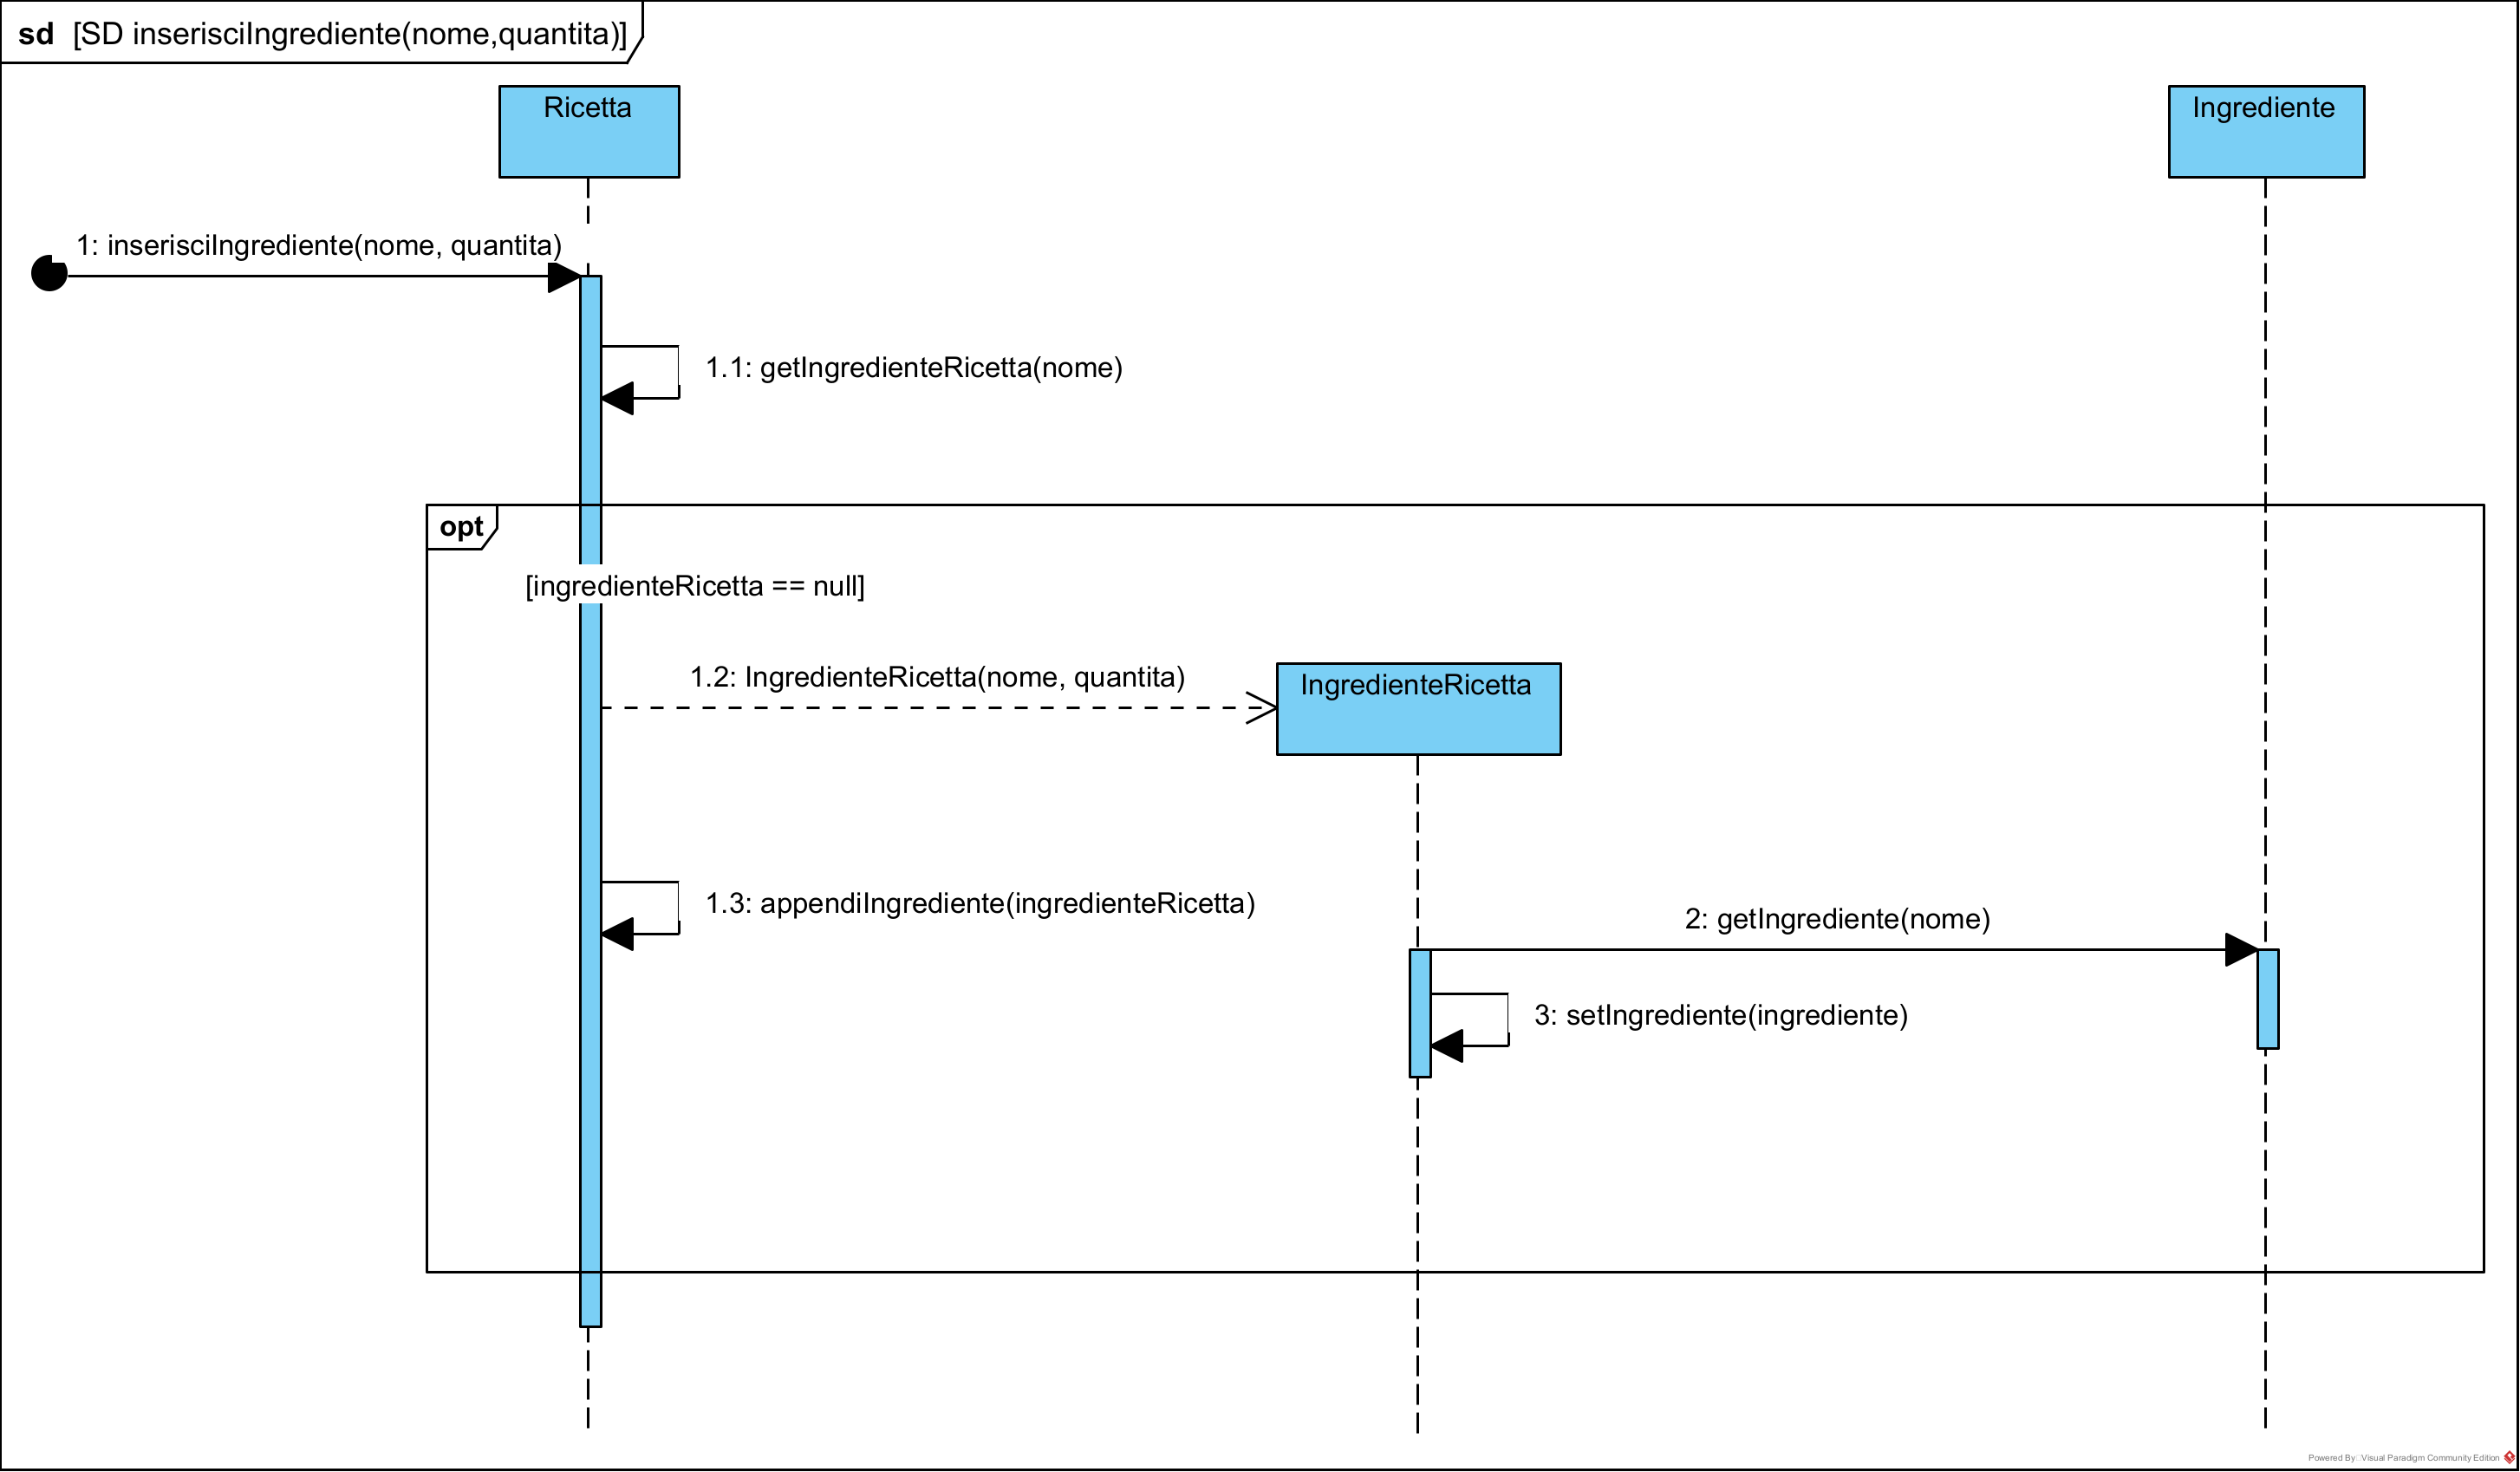
\includegraphics[width=01\linewidth]{image/SD-inserisciIngrediente.png}
				\caption{SD - inserisciIngrediente}\label{fig:SD-inserisciIngrediente}
			\end{figure}

         \section{Diagramma degli Stati}
         E' stato realizzatto il diagramma degli stati della entità Birra per descrivere le modifiche dinamiche degli stati dell'entità stessa (figura \ref{fig:stati-birra}).
		\begin{figure}[!h]
			\centering
			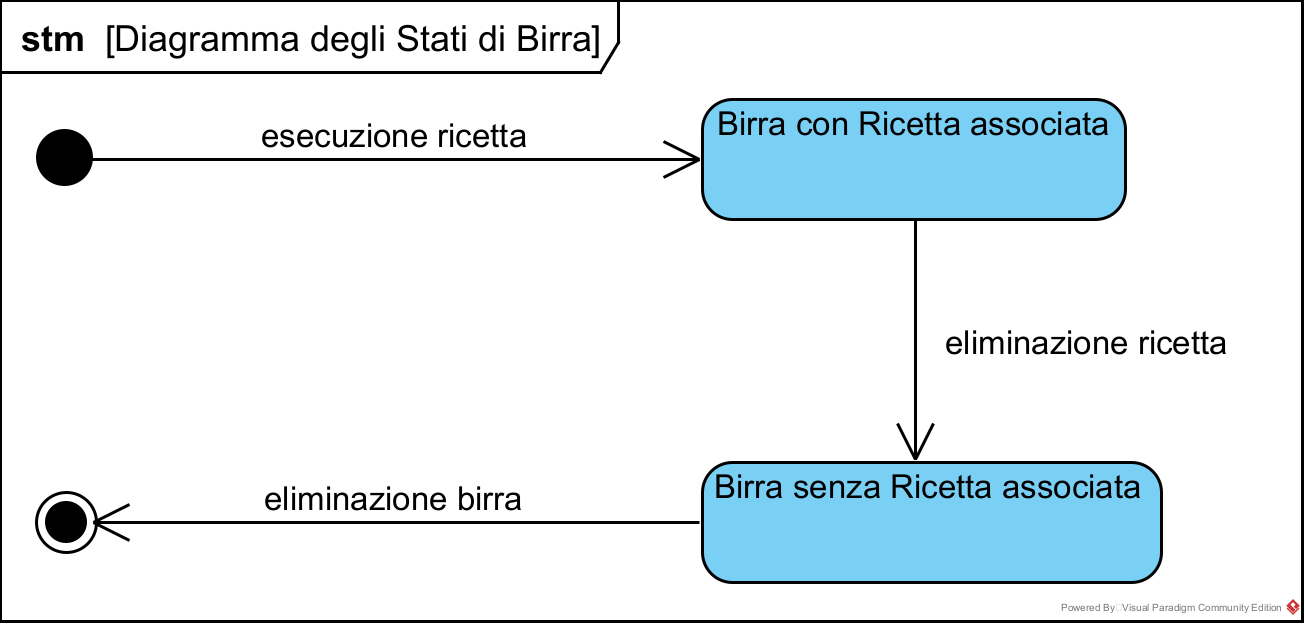
\includegraphics[width=0.8\linewidth]{image/Diagramma-degli-Stati-Birra.png}
			\caption{Diagramma degli Stati Birra}\label{fig:stati-birra}
		\end{figure}    			

         \section{Diagramma delle Attività }
         E' stato realizzatto il diagramma delle attività per descrivere il processo di esecuzione di una ricetta (figura \ref{fig:attivita-esegui-ricetta}).
		\begin{figure}[!h]
			\centering
			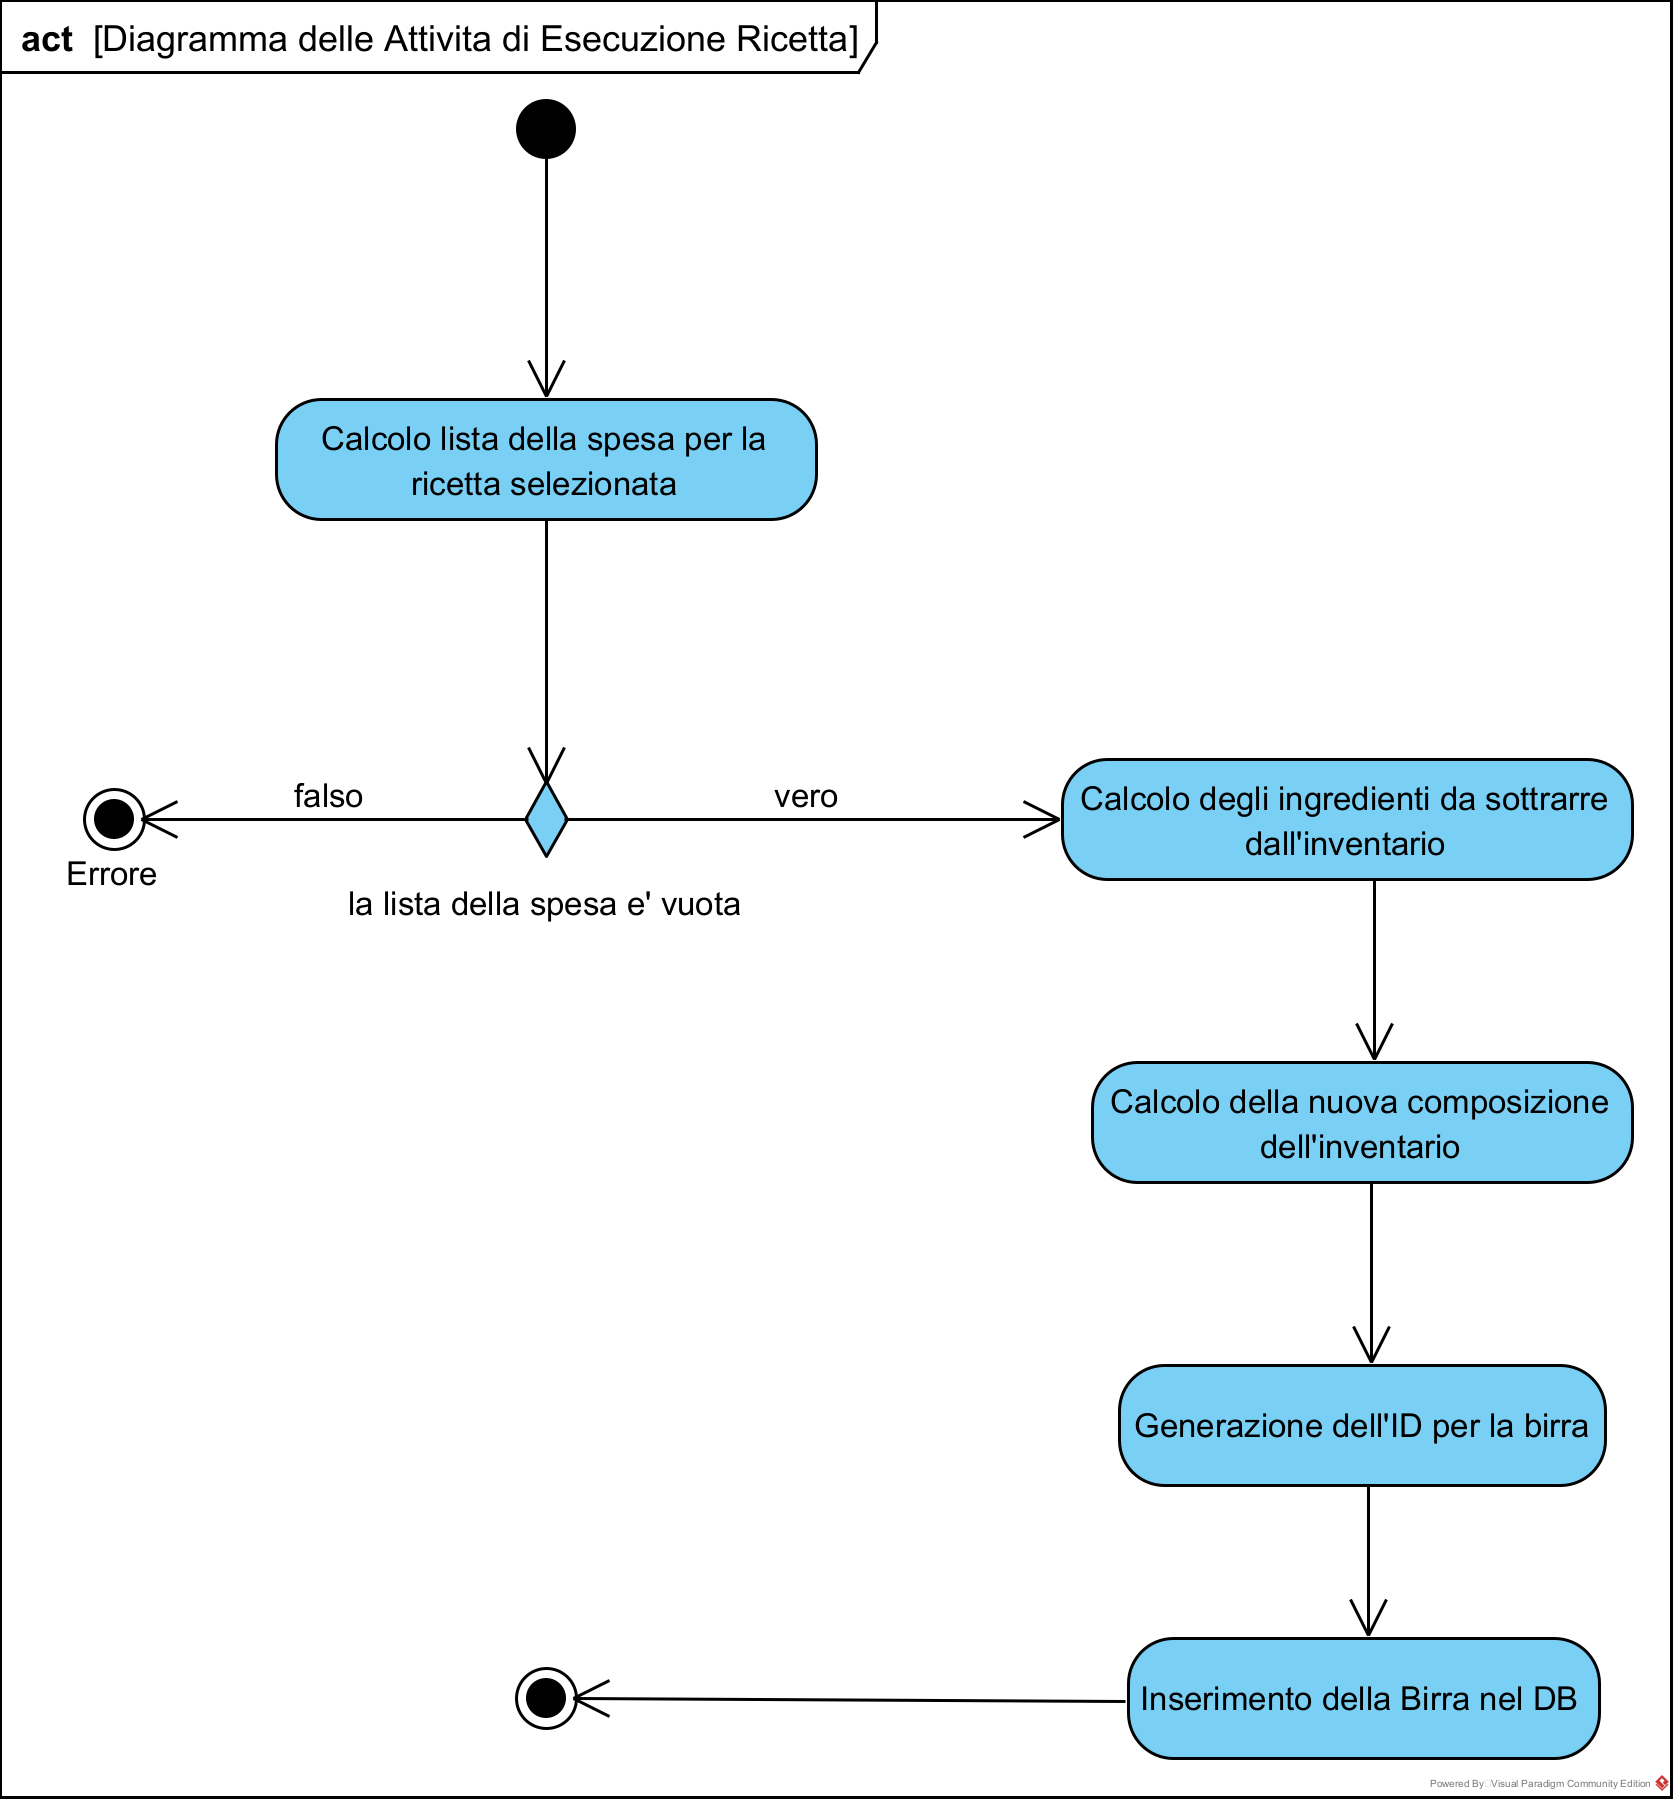
\includegraphics[width=0.6\linewidth]{image/Diagramma-delle-Attivita-di-Esecuzione-Ricetta.png}
			\caption{Diagramma delle Attivita di Esecuzione Ricetta}\label{fig:attivita-esegui-ricetta}
		\end{figure}    
\newpage	
      	\section{Pattern Utilizzati}		
	Nel corso delle fasi di progettazione, implementazione e refactoring abbiamo individuato dei pattern archietturali e dei design pattern. 
	      	\subsection{Pattern Architetturali}
		
			\subsubsection{Page Controller}
			Le classi Endpoint rappresentano una divisione in pagine dell'API, quindi sono un'applicazione del pattern architetturale Page Controller.	
			
			\subsubsection{Table Data Gateway}
Tutte le interfacce Repository implementano pattern architetturale Table Data Gateway, in quanto rappresentano un'interfaccia unificata e fruibile per ottenere informazioni dalla tabella di database che può essere remoto o locale.	
      		
		
		\subsection{Design Pattern}
			\subsubsection{Chain of Responsibility}
			Le classi Validator e ValidatorHandler (e derivate) implementano il design pattern Chain of Responsibility, in quanto la validazione dei campi è delegata a catene di ValidatorHandler che eseguono controlli ed eventualmente lanciano una eccezione ValidationException.
		
			\subsubsection{Singleton}	
			Tutti i controller (tranne ControllerResetController) implementano il design pattern Singleton, quindi hanno tutti rispettivamente l'istanza statica instance, il metodo statico createInstance che assegna ad ogni controller la sua istanza statica (creata e coordinata da ControllerResetController) e il metodo getInstance.
Tutte le interfacce Repository hanno associato rispettivamente una classe utility nominata RepositoryGateway, una classe che usa il pattern singleton per avere solo una istanza dei repository JDBC.
Implementano questo pattern anche le classi Validator, ValidatorHandler e le classi IDGenerator e derivate. 
				
		\subsubsection{Strategy, Template Method}
		Le classi IDGenerator e derivate implementano i pattern Strategy e Template Method dal momento che IDGenerator definisce la successione delle fasi preprocess -> compute -> postprocess, le quali sono modificabili singolarmente dalle derivate, e perchè le derivate applicano potenzialmente algoritmi diversi per ottenere lo stesso risultato. 
		
		\subsubsection{Facade}		
		La classe IDGenerationFacade è applicazione dei design pattern Facade.

      \chapter{Implementazione}
      
      \section{Scelte Implementative - Backend}
Per realizzare il backend abbiamo deciso di utilizzare Spring, framework open source per lo sviluppo di applicazioni su piattaforma Java.
Come interfaccia per il database abbiamo usato CrudRepository.\\
   	\section{Scelte Implementative - Frontend}
Per realizzare l'interfaccia utente abbiamo deciso di utilizzare la libreria open-source React, la quale utilizza come linguaggio JavaScript/JSX.
							
      \chapter{Conclusioni}
    
     	\section{Analisi con SonarQube e SonarCloud}
Durante le fasi di implementazione abbiamo utilizzato il tool SonarQube e la gitHub Action che automatizza l'analisi con SonarCloud per mantenere controllato il livello di qualità del progetto.\\

		\begin{figure}[!h]
			\centering
			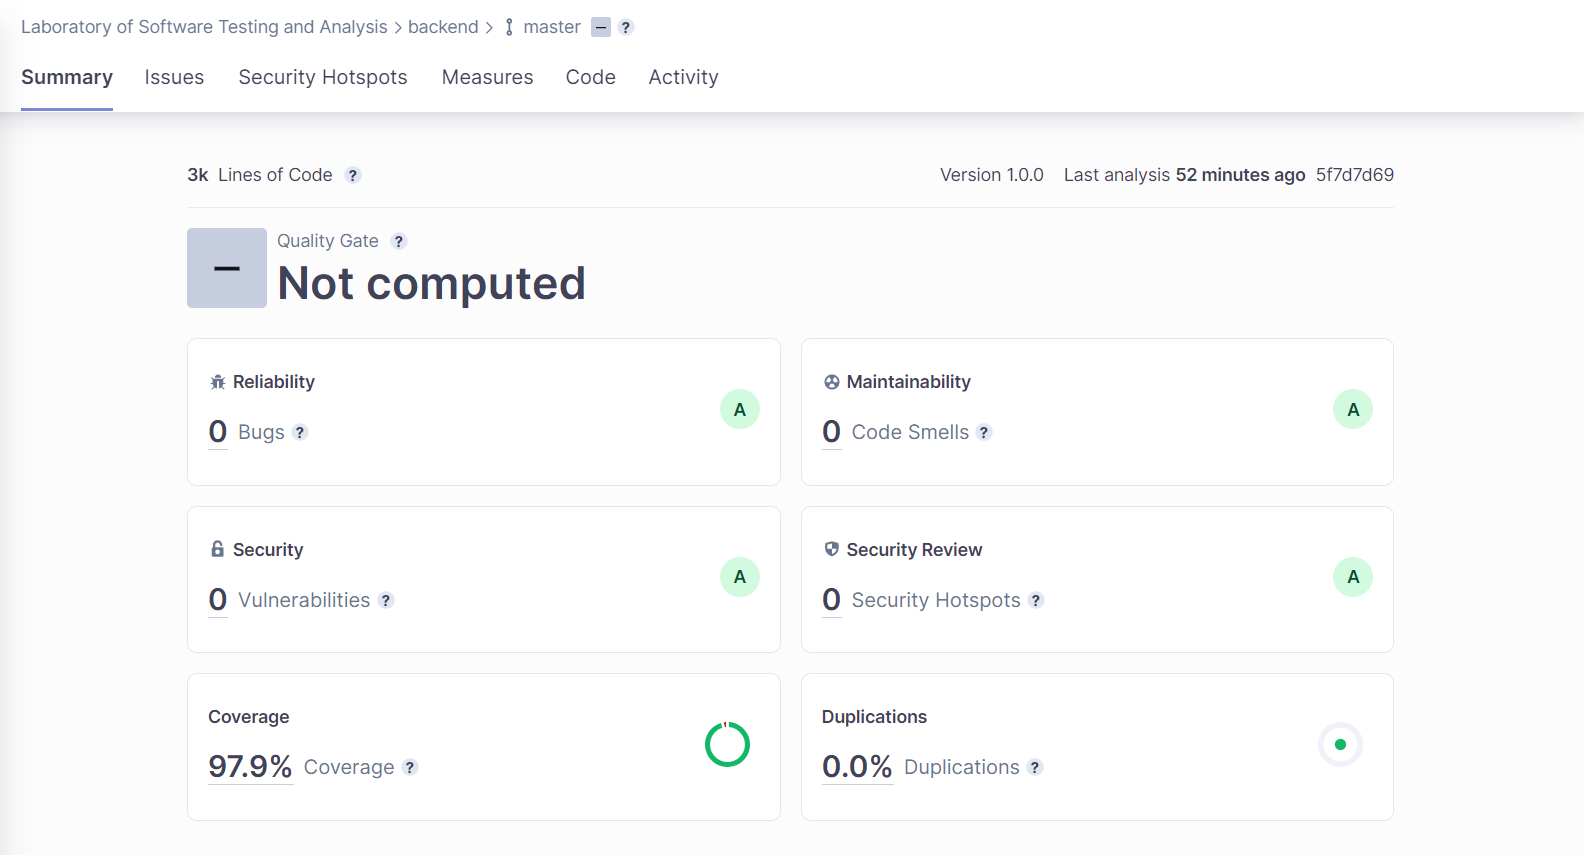
\includegraphics[width=1\linewidth]{image/sonarCloud-backend.png}
			\caption{sonarCloud-backend}\label{fig:sonarCloud-backend}
		\end{figure}	
		\begin{figure}[!h]
			\centering
			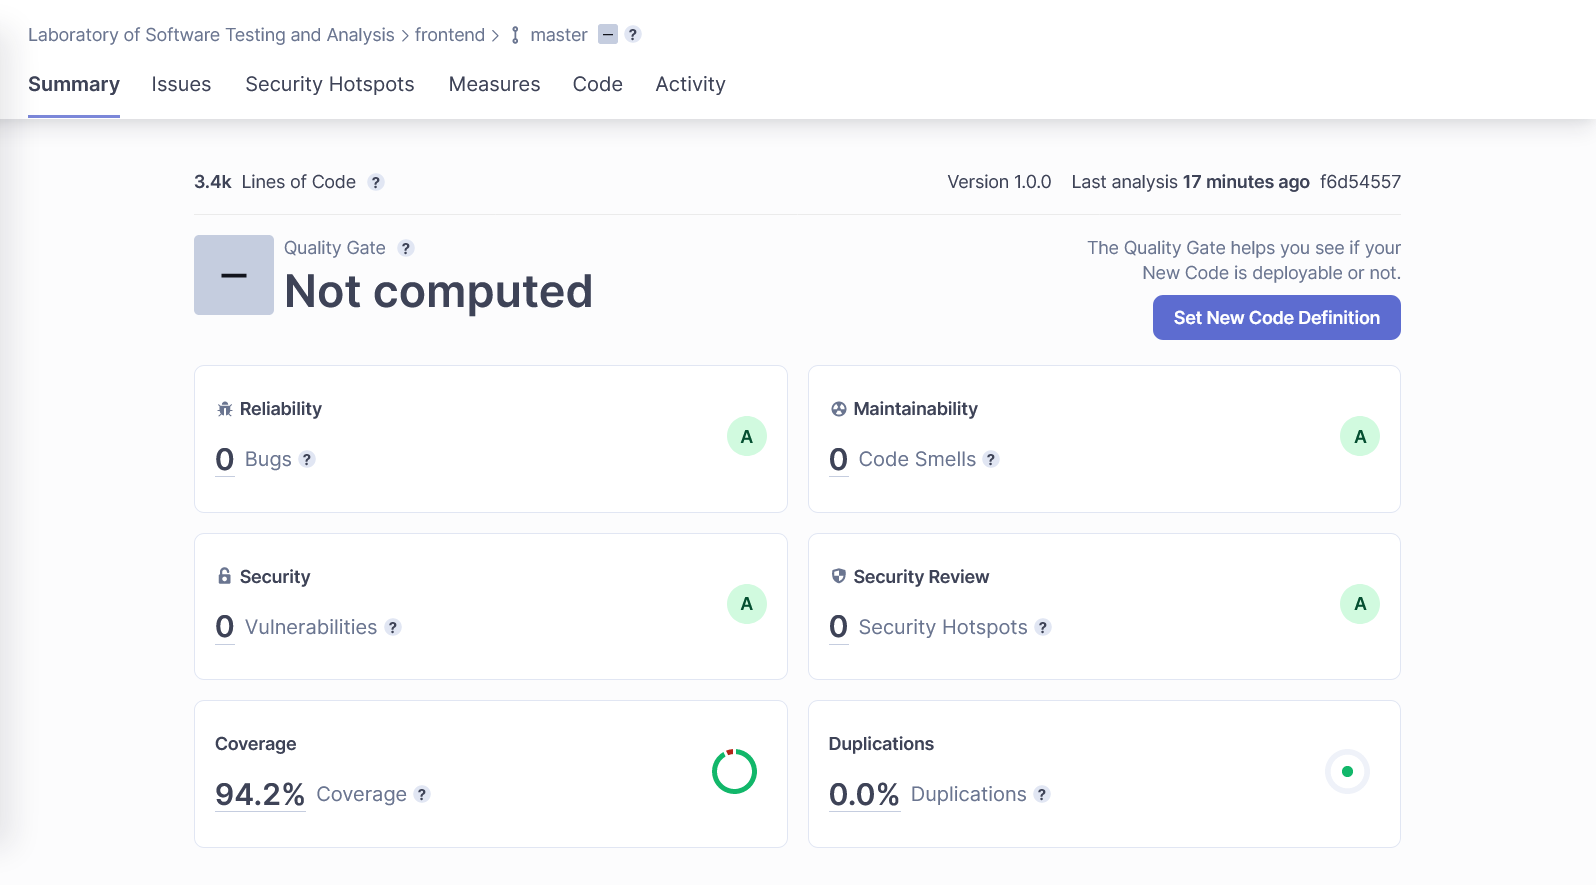
\includegraphics[width=1\linewidth]{image/sonarCloud-frontend.png}
			\caption{sonarCloud-frontend}\label{fig:sonarCloud-frontend}
		\end{figure}
		\newpage 
Dalle analisi finali svolte, i cui risultati sono riportati nelle figure \ref{fig:sonarCloud-backend} e \ref{fig:sonarCloud-frontend}, si può affermare che il progetto non presenta bugs, code Smells, vulnerabilità e problemi di sicurezza.\\
Utilizzando i test JUnits per il backend e Jest per il frontend, siamo inoltre riusciti ad ottenere una coverage elevata del codice, pari al 97.8\% nel backed e del 94.2\% nel frontend.


\newpage
      	\section{Analisi con Understand}
	Abbiamo utilizzato il tool Understand per capire se nel progetto fossero presenti anti-pattern strutturali legati a problemi di dipendenza o altri problemi.\\
Secondo un'analisi generale (figura \ref{fig:understand}) si può intuire come il progetto sia privo di problemi e presenti una struttura ben bilanciata.\\
Sono stati realizzati i grafici metrici per le classi e i metodi sia del front-end (figura \ref{fig:F-Classi} e \ref{fig:F-Metodi}) sia per il back-end (figura \ref{fig:B-Classi} e \ref{fig:B-Metodi}).\\
Nei grafici la grandezza rappresenta il numero di istruzioni, mentre il colore la complessità ciclomatica.\\
		\begin{figure}[!h]
			\centering
			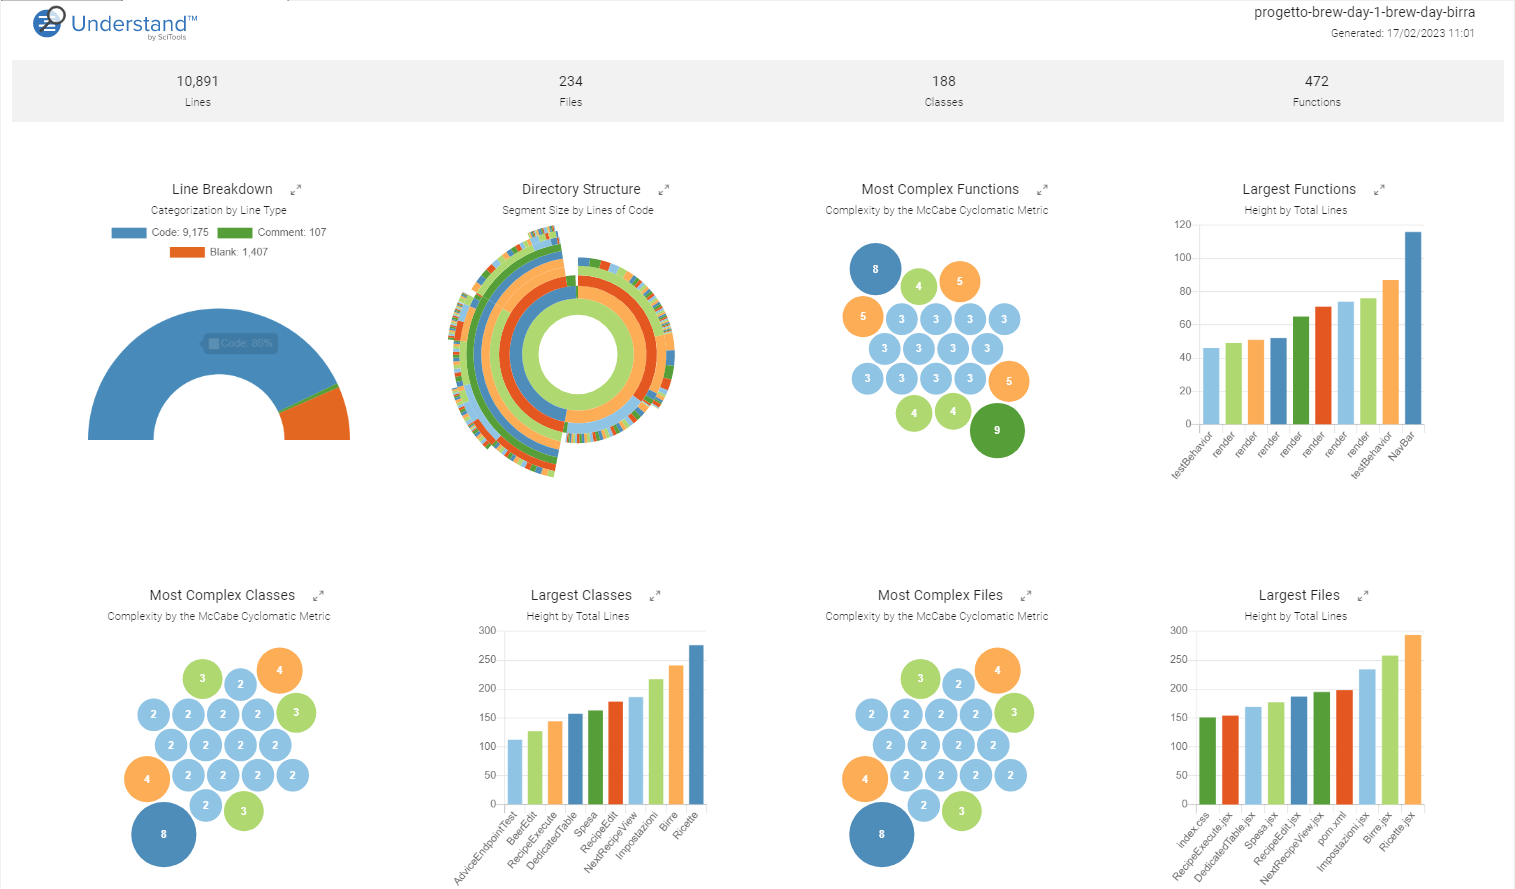
\includegraphics[width=1\linewidth]{image/understand.png}
			\caption{Understand}\label{fig:understand}
		\end{figure}
		
		\begin{figure}[!h]
			\centering
			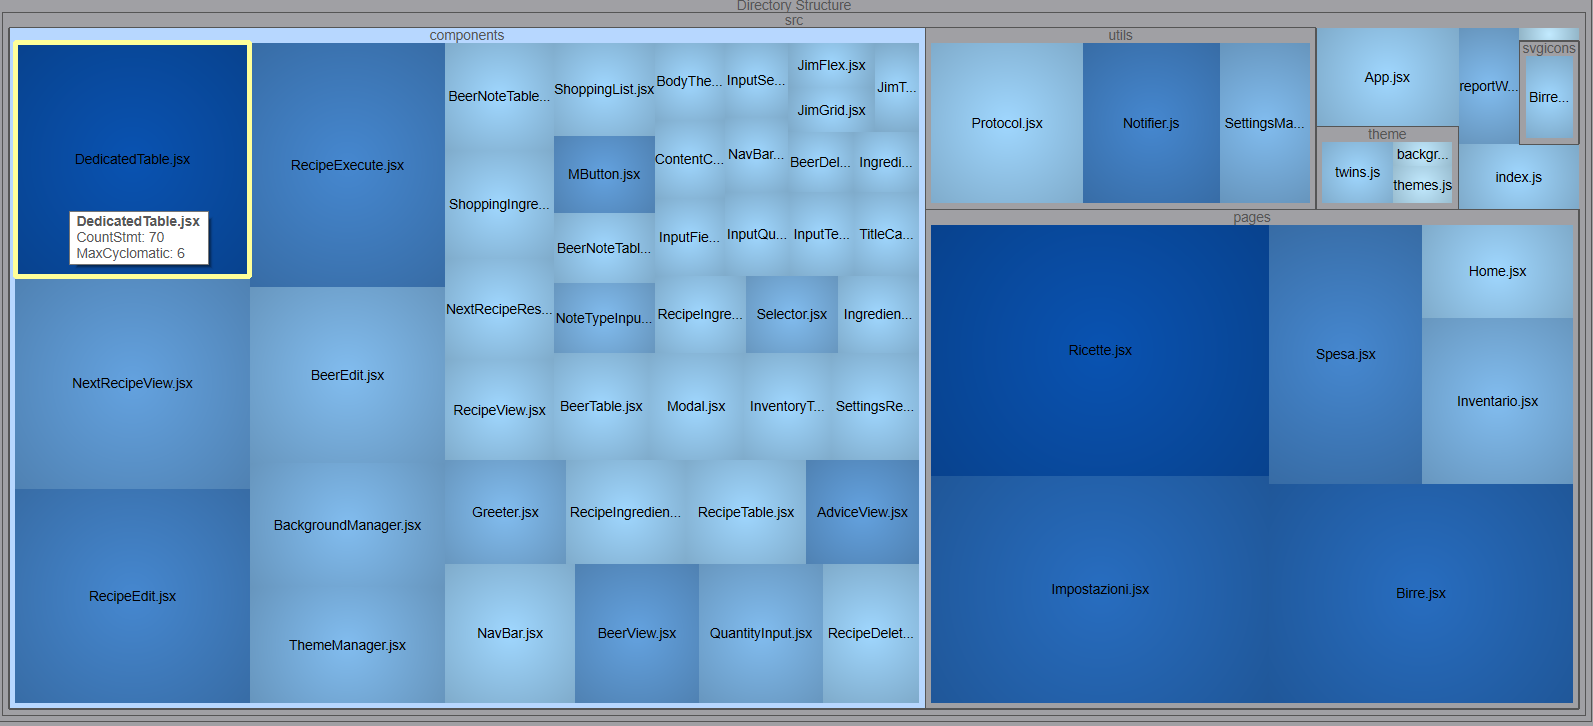
\includegraphics[width=1\linewidth]{image/F-Classi.png}
			\caption{Mappatura per Classi - Frontend}\label{fig:F-Classi}
		\end{figure}    

		\begin{figure}[!h]
			\centering
			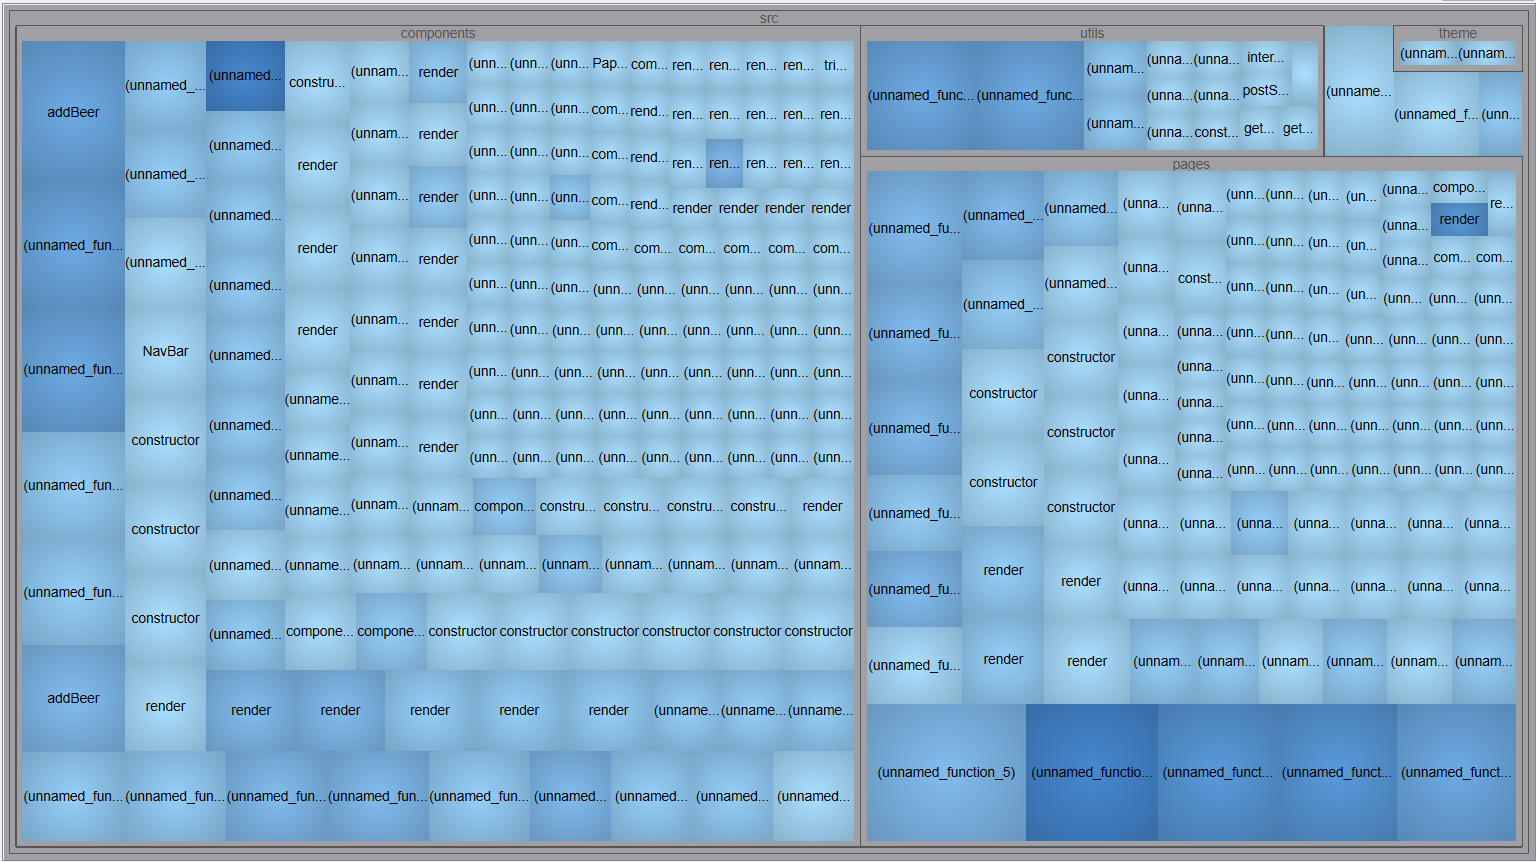
\includegraphics[width=0.9\linewidth]{image/F-Metodi.png}
			\caption{Mappatura per Metodi - Frontend}\label{fig:F-Metodi}
		\end{figure}    

		\begin{figure}[!h]
			\centering
			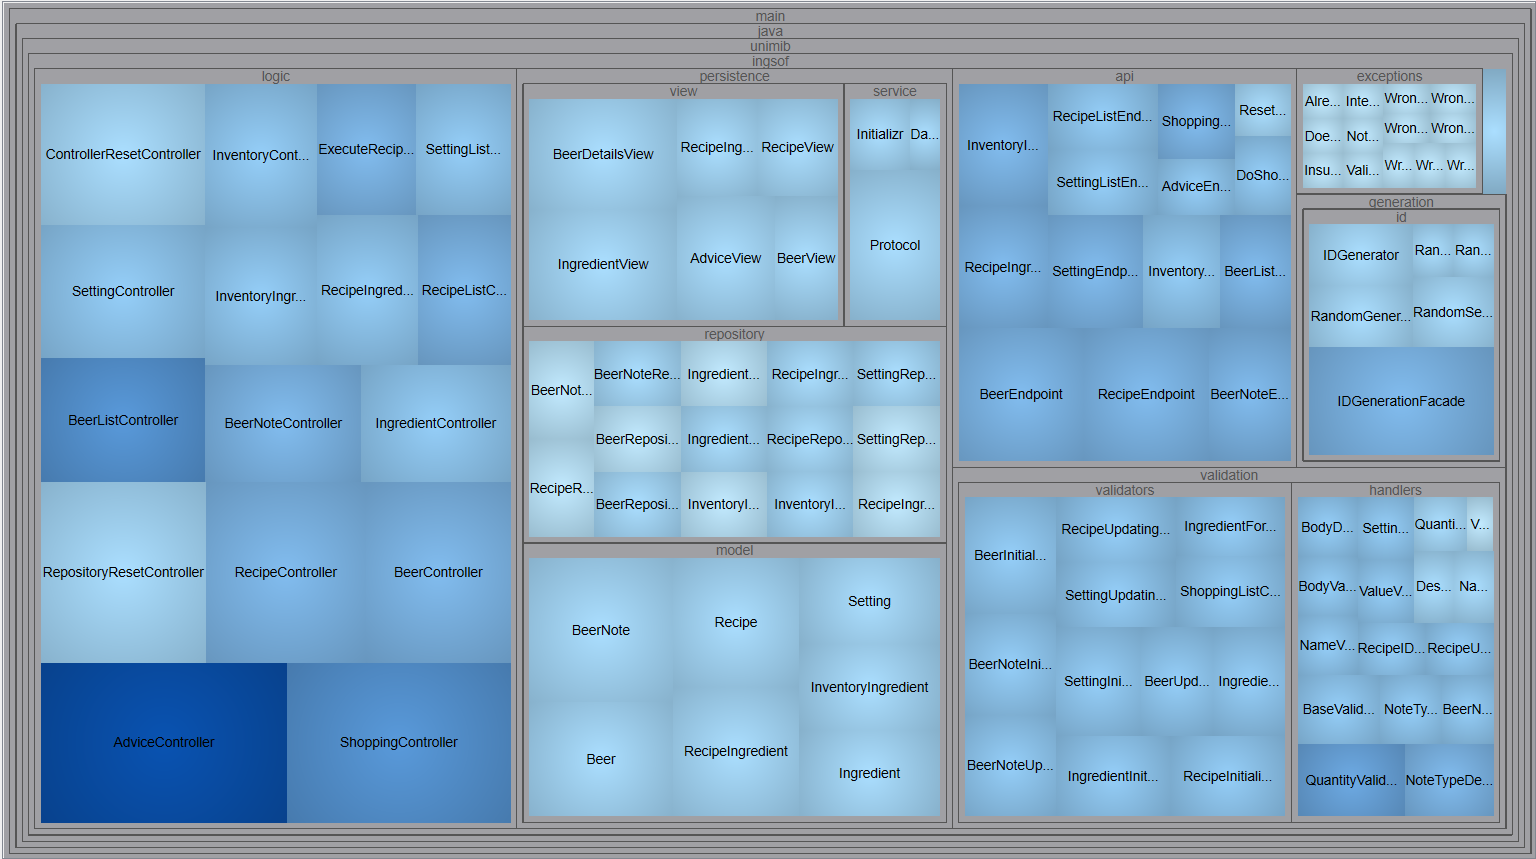
\includegraphics[width=0.9\linewidth]{image/B-Classi.png}
			\caption{Mappatura per Classi - Backend}\label{fig:B-Classi}
		\end{figure}    

		\begin{figure}[!h]
			\centering
			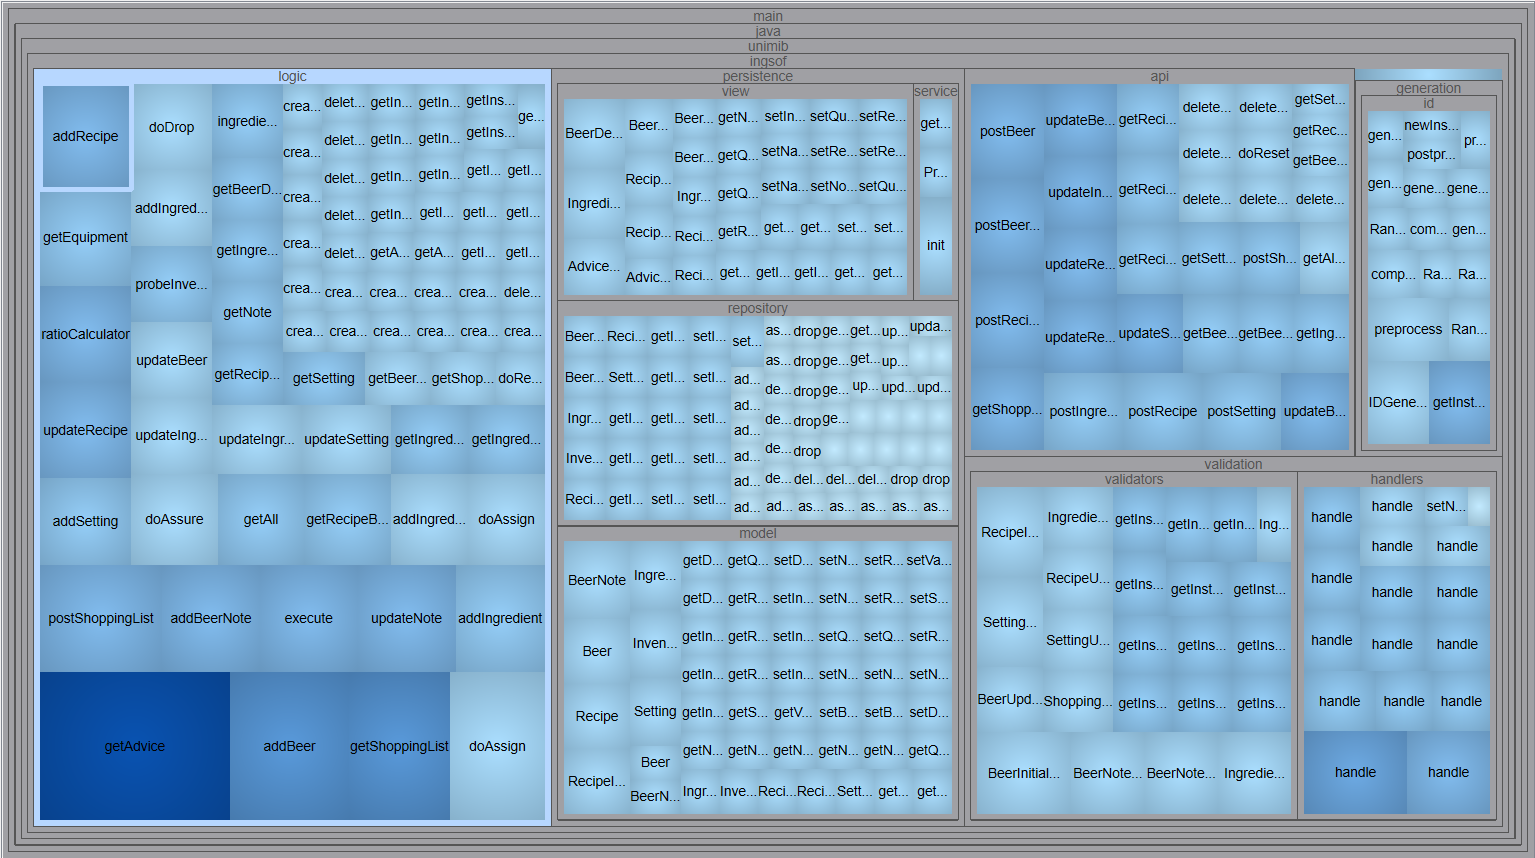
\includegraphics[width=0.9\linewidth]{image/B-Metodi.png}
			\caption{Mappatura per Metodi - Backend}\label{fig:B-Metodi}
		\end{figure}    
	
		 	
	\section{Considerazioni Finali}
Consideriamo il progetto completo nelle funzionalità richieste.\\
Con questo progetto abbiamo potuto realizzare un'applicazione lavorando in team e andando a coprire tutte le fasi, dall'analisi, la progettazione, l'implementazione, il refactoring, fino al rilascio.\\
Siamo soddisfatti di come abbiamo lavorato in gruppo dal momento che siamo sempre riusciti a comunicare e ad avere le idee chiare su ciò che andava fatto. Tutto ciò è stato semplificato dall'utilizzo del framework Scrum e l'uso proficuo di gitHub.\\
Abbiamo avuto la possibilità di mettere in pratica le conoscenze di gestione del progetto acquisite da ogni componente del gruppo durante il corso di Analisi e Progettazione del Software e di Ingegneria del Software, oltre ad altri corsi per quanto riguarda l'implementazione.\\
 
	
	
 	\section{Link Utili}  
	\href{https://github.com/lta-unimib/progetto-brew-day-1-brew-day-birra}{Repository githHub}\\
	\href{https://github.com/lta-unimib/progetto-brew-day-1-brew-day-birra/wiki}{Wiki su gitHub}\\
	\href{https://github.com/lta-unimib/progetto-brew-day-1-brew-day-birra/wiki/Installazione-Guidata}{Installazione Guidata}\\
	\href{https://github.com/lta-unimib/progetto-brew-day-1-brew-day-birra/wiki/Uso-dell'Applicazione}{Uso dell'Applicazione}\\
	\href{https://github.com/lta-unimib/progetto-brew-day-1-brew-day-birra/tree/master/backend#readme}{Documentazione Api}\\
	\href{https://github.com/lta-unimib/progetto-brew-day-1-brew-day-birra/tree/master/scrum}{Documentazione Scrum}\\

\end{document}
